\documentclass[11pt, a4paper]{article}

% --- PRÉAMBULE SIMPLIFIÉ ET ROBUSTE ---
\usepackage[ruled,vlined,french]{algorithm2e}
\usepackage[utf8]{inputenc}
\usepackage[T1]{fontenc}
\usepackage[french]{babel}
\usepackage[a4paper, top=2.5cm, bottom=2.5cm, left=2cm, right=2cm]{geometry}
\usepackage{amsmath}
\usepackage{enumitem}
\usepackage{graphicx}
\usepackage{float}
\usepackage{subcaption}
\usepackage{booktabs}
\usepackage{tabularx}

\setlist[itemize]{label=-}

\begin{document}

% --- PAGE DE GARDE ---
\begin{titlepage}
    \centering
    \vspace*{1cm}
    
    \Large \textsc{Université de Caen Normandie} \\
    \large Licence Informatique -- 3\textsuperscript{ème} année (L3) \\
    \large Matière : Projet 2
    
    \vspace{3cm}
    
    \Huge
    \textbf{Dota 2 Trajectory Analyzer}
    
    \vspace{0.5cm}
    \LARGE
    Fouille de Motifs Spatio-Temporels et Clustering de Trajectoires E-sport pour en extraire les stratégies
    
    \vspace{1.5cm}
    
    \textbf{Rapport de Projet de Conception}
    
    \vspace{2.5cm}
    
    \Large
    \textbf{Équipe de développement :} \\
    \vspace{0.5cm}
    Elias \textsc{Okat} \\
    Uzay \textsc{Turkmenel} \\
    Paul \textsc{Aubert}
    
    \vfill
    
    \Large
    \textbf{Année universitaire 2025-2026}
    
    \vspace{1cm}
\end{titlepage}

% --- SOMMAIRE ---
\tableofcontents
\newpage

% ==========================================
% SECTION 1 : INTRODUCTION
% ==========================================
\section{Introduction}

\subsection{Description Générale du Projet}

L'avènement de l'e-sport (sport électronique) a généré des volumes de données sans précédent. Dans des jeux compétitifs complexes comme \textit{DotA 2} (Defense of the Ancients 2), chaque partie génère des dizaines de milliers de points de données spatio-temporelles, reflétant les moindres clics et déplacements des joueurs. Si ces données brutes sont massivement stockées, leur exploitation stratégique reste un défi majeur pour les analystes et les équipes professionnelles.

Ce projet s'inscrit dans cette dynamique d'analyse automatique de données de jeu appliquée à l'e-sport. Notre objectif est de concevoir et d'implémenter une chaîne de traitement algorithmique capable d'ingérer les trajectoires brutes des joueurs pour en extraire des régularités de mouvement et des stratégies partielles interprétables. 

\subsection{Plan du Rapport}

Ce rapport détaillera l'intégralité de notre démarche. Après avoir exposé les objectifs et la problématique du projet (Section 2), nous décrirons les fonctionnalités implémentées et l'organisation de l'équipe (Section 3). Nous présenterons ensuite les éléments techniques et algorithmiques (Section 4) ainsi que l'architecture logicielle du système (Section 5). Nous consacrerons une large partie à l'évaluation expérimentale de nos modèles --- de la compression géométrique au clustering spatial, jusqu'à l'extraction finale des motifs stratégiques (Section 6). Enfin, nous conclurons sur les apports de ce projet et ses perspectives d'évolution (Section 7).

% ==========================================
% SECTION 2 : OBJECTIFS DU PROJET
% ==========================================
\section{Objectifs du Projet}

\subsection{Contexte Métier : Le Jeu DotA 2}
\textit{DotA 2} est un jeu vidéo de type MOBA (Multiplayer Online Battle Arena). Deux équipes de cinq joueurs s'affrontent sur une carte fermée et asymétrique, composée de trois voies principales (les \textit{Lanes}), séparées par une rivière et des zones de forêts (la \textit{Jungle}). L'objectif est de détruire la base adverse. La victoire repose non seulement sur les réflexes mécaniques (micro-gestion), mais surtout sur la prise de décision globale, les déplacements coordonnés et le contrôle de la carte (macro-gestion).

\subsection{La Problématique de l'Analyse de Trajectoires}
La donnée brute dont nous disposons est un flux continu de coordonnées $(X, Y)$ enregistrées à intervalles réguliers (les \textit{ticks}). Cette donnée pose trois problèmes majeurs :
\begin{enumerate}
    \item \textbf{Le volume :} Une partie génère des millions de points.
    \item \textbf{Le bruit stochastique :} Les joueurs cliquent frénétiquement pour maintenir leur personnage en mouvement (micro-tremblements), générant un nuage de points erratique qui ne représente aucune réelle intention de déplacement.
    \item \textbf{L'absence de sémantique :} Un point $(120, 115)$ n'a aucun sens stratégique pour une machine.
\end{enumerate}

L'objectif fondamental de ce projet est donc de répondre à la question scientifique suivante : \textbf{Comment transformer de manière non supervisée un volume massif de micro-clics erratiques en un alphabet de comportements locaux (ganks, farming, rotations) compréhensible par un analyste humain ?}

\subsection{Points-Clés et Grandes Étapes}

Le cœur mathématique du projet repose sur un pipeline de données séquentiel en trois phases :
\begin{enumerate}
    \item \textbf{Phase 1 - Compression (MDL) :} Nettoyage des nuages de points erratiques pour extraire des segments de droites directionnels.
    \item \textbf{Phase 2 - Discrétisation Spatiale (TRACLUS + AP) :} Calcul de la matrice de similarité entre les segments, puis clustering pour découvrir les "Macro-Zones" de la carte.
    \item \textbf{Phase 3 - Extraction Sémantique (PrefixSpan) :} Recodage des trajectoires en séquences d'états (via Run-Length Encoding) et fouille de motifs fréquents pour identifier les véritables stratégies (ex: zone A $\rightarrow$ zone B $\rightarrow$ zone C).
\end{enumerate}

\subsection{Travaux Existants et Positionnement}

L'analyse des déplacements dans les jeux vidéo compétitifs a fait l'objet de plusieurs approches académiques dans le domaine du \textit{Game Analytics} \cite{drachen}. Pour extraire de l'information stratégique à partir de coordonnées spatiales, la littérature s'appuie généralement sur trois grandes méthodologies, qui présentent cependant certaines limites face à la complexité de \textit{DotA 2} :

\begin{enumerate}
    \item \textbf{La cartographie statistique statique (Heatmaps) :}
    L'approche la plus répandue dans l'industrie consiste à agréger les positions des joueurs pour générer des cartes de chaleur. Si cette méthode permet d'identifier visuellement les zones de forte activité, elle écrase totalement la dimension temporelle et séquentielle. Une \textit{heatmap} montre qu'un joueur a été dans la jungle puis au centre, mais ne permet pas de savoir s'il s'agit d'une rotation offensive ou d'un repli.

    \item \textbf{L'analyse séquentielle sur grilles prédéfinies :}
    Pour réintégrer le temps, de nombreux travaux d'analyse de trajectoires standards \cite{zheng} découpent arbitrairement la carte en une grille mathématique ou utilisent les zones sémantiques codées en dur dans le jeu. Les trajectoires sont alors converties en séquences de zones. La limite majeure de cette approche est le \textbf{biais humain} : le découpage manuel ne correspond pas nécessairement aux véritables flux de déplacement des joueurs, générant du bruit aux frontières arbitraires.

    \item \textbf{Le clustering direct par Dynamic Time Warping (DTW) :}
    D'autres études tentent de comparer directement les trajectoires brutes en utilisant des métriques de distance temporelles flexibles comme le DTW ou la distance de Fréchet. Bien que mathématiquement robustes, ces méthodes se heurtent au mur de la scalabilité ($\mathcal{O}(N^2)$ voire $\mathcal{O}(N^3)$) sur des millions de points et sont extrêmement sensibles aux micro-tremblements de la souris.
\end{enumerate}

\textbf{Positionnement de notre étude :} 
Notre projet se démarque de ces approches par la conception d'un pipeline \textbf{hybride et totalement guidé par la donnée (\textit{data-driven})}. 
Pour contourner les limites du DTW et de l'échantillonnage classique, nous nous appuyons sur le paradigme \textit{Partition-and-Group} introduit par Lee et al. \cite{lee2007}. Nous supprimons le bruit en amont via leur algorithme de compression géométrique \textbf{MDL}. Ensuite, contrairement au découpage arbitraire en grille, notre zonage est découvert dynamiquement de manière non supervisée par l'algorithme \textbf{Affinity Propagation} combiné à la distance experte \textbf{TRACLUS} \cite{lee2007}. Enfin, l'application de l'algorithme \textbf{PrefixSpan}, formalisé par Pei et al. \cite{pei2001}, sur cet alphabet purifié permet de retrouver la dynamique temporelle perdue par les simples \textit{Heatmaps}.

% ==========================================
% SECTION 3 : FONCTIONNALITÉS IMPLÉMENTÉES
% ==========================================
\section{Fonctionnalités Implémentées}

Le projet a été développé pour être utilisable à la fois par des ingénieurs (via une CLI offrant 11 commandes d'automatisation et de batching) et par des analystes finaux via une Interface Graphique (GUI) avancée (v1.1.0).

\subsection{Description des Fonctionnalités}

Conçue avec le framework \textit{CustomTkinter} selon le patron de conception MVC (Modèle-Vue-Contrôleur), l'application propose un environnement ergonomique structuré autour de 7 modules interactifs :

\begin{itemize}
    \item \textbf{Accueil (Dashboard) :} Un tableau de bord dynamique présentant les métriques clés de la base de données en temps réel (Matchs ingérés, Matchs compressés, Clusters générés, Motifs fréquents extraits).
    
    \item \textbf{Overlay Carte et Exploration spatiale :} Outil de visualisation superposant les trajectoires sur la carte officielle de \textit{DotA 2}. Il intègre un filtrage granulaire et un curseur temporel permettant d'inspecter les déplacements \textit{tick par tick}.
    
    \item \textbf{Module de Compression (MDL) :} Interface de traitement par lots intégrant un suivi en temps réel via une console de \textit{logs} (taux de réduction, empreinte mémoire).
    
    \item \textbf{Atelier de Clustering :} Espace d'exploration permettant de paramétrer les algorithmes spatiaux. L'interface s'adapte dynamiquement à l'algorithme choisi (ex: sélection du \textit{damping} pour l'AP) et affiche le pavage spatial généré.
    
    \item \textbf{Comparateur Synchronisé (Brut vs Compressé) :} Module d'inspection visuelle affichant deux cartes côte à côte. Le système pré-calcule l'intégralité des \textit{frames} en mémoire pour garantir une lecture temporelle parfaitement fluide et synchronisée.
    
    \item \textbf{Fouille Séquentielle (PrefixSpan) :} Interface dédiée à l'extraction sémantique restituant les résultats sous forme de tableau textuel filtrable, d'histogramme des fréquences, et de graphe de transitions interactif.
    
    \item \textbf{Orchestrateur End-to-End (Pipeline) :} Module automatisant la chaîne de valeur. L'exécution parallèle s'appuie sur le \textit{multiprocessing} natif ($\text{CPU\_count} - 2$ cœurs). Des indicateurs visuels suivent l'avancement des étapes jusqu'à la génération des résultats analytiques finaux.
\end{itemize}

\subsection{Qualité Logicielle}
Le projet est accompagné d'une suite de \textbf{72 tests unitaires} couvrant l'ensemble des modules critiques (compression, géométrie, clustering, fouille de motifs). Ces tests sont exécutables via \texttt{pytest} et permettent de vérifier systématiquement le bon fonctionnement du pipeline après chaque modification du code.

\subsection{Organisation du Projet : Répartition des Tâches}
Le développement de ce projet a nécessité une répartition des rôles au sein de notre groupe de trois étudiants :
\begin{itemize}
    \item \textbf{Elias OKAT} : Parsing des fichiers CSV bruts avec Pandas, implémentation de l'algorithme de compression MDL, K-Médoïdes pour le clustering et implémentation des benchmarks pour MDL et clustering.
    \item \textbf{Uzay TURKMENEL} : Calculs géométriques vectorisés (distances TRACLUS) et développement des algorithmes de clustering spatiaux.
    \item \textbf{Paul AUBERT} : Recodage RLE, développement \textit{from scratch} de l'algorithme PrefixSpan et modélisation sous forme de Graphe de Markov.
\end{itemize}

% ==========================================
% SECTION 4 : ÉLÉMENTS TECHNIQUES
% ==========================================
\section{Éléments Techniques}

\subsection{Description des Données}

Nos expérimentations portent sur un corpus de 70 matchs réels de \textit{DotA 2} (fichiers CSV), représentant 10 joueurs par match. Chaque fichier contient un \textit{tick} par ligne avec les coordonnées $(X,Y)$ des 10 joueurs. Après compression avec $w_{error}=12$, ce corpus génère environ 18\,000 segments. Pour l'étape de fouille de motifs (Section 6.4), un sous-ensemble de 30 matchs est utilisé, produisant 1\,174 séquences fréquentes avec un support minimum de $15\%$.

Pour illustrer la transformation opérée par notre pipeline, la Figure \ref{fig:data_transition} présente la transition entre la donnée brute et la donnée structurée :

\begin{figure}[H]
    \centering
    \begin{subfigure}[t]{0.48\textwidth}
        \centering
        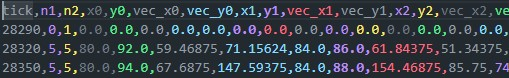
\includegraphics[width=\linewidth, height=0.25\textheight, keepaspectratio]{img/extrait_csv.jpg}
        \caption{Extrait du flux brut (CSV).}
        \label{fig:csv_brut}
    \end{subfigure}\hfill
    \begin{subfigure}[t]{0.48\textwidth}
        \centering
        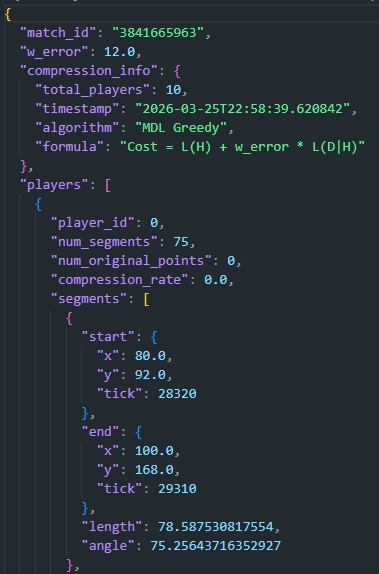
\includegraphics[width=\linewidth, height=0.25\textheight, keepaspectratio]{img/json_extrait.jpg}
        \caption{Séquence encodée après traitement.}
        \label{fig:seq_encodee}
    \end{subfigure}
    \caption{Transition entre la donnée brute et la donnée structurée par le pipeline.}
    \label{fig:data_transition}
\end{figure}

\subsection{Description des Algorithmes : Pseudo-code MDL Compress}

L'algorithme glouton (Greedy) inspiré du principe du Minimum Description Length (MDL) \cite{rissanen1978}, tel qu'adapté par Lee et al. \cite{lee2007} pour la simplification de trajectoires, est la clé de voûte du débruitage. Son implémentation vectorisée en \texttt{NumPy} permet d'accélérer significativement le traitement. 

\textbf{Note terminologique :} Notre implémentation s'inspire du critère MDL tel que décrit par Lee et al. \cite{lee2007}, où le coût d'encodage est simplifié sous la forme d'un seuil de distance perpendiculaire ($w_{error}$). Il ne s'agit pas d'une implémentation complète du principe MDL au sens de Rissanen \cite{rissanen1978} (minimisation de $L(H) + L(D|H)$), mais d'une approximation pratique qui conserve l'idée de compromis entre concision et fidélité.

\begin{algorithm}[H]
\DontPrintSemicolon
\KwIn{$T = [p_1, p_2, \dots, p_n]$ (liste ordonnée des coordonnées du joueur) \newline
      $w_{error}$ (seuil de tolérance de distance perpendiculaire max)}
\KwOut{$S$ (liste des segments compressés)}
$S \leftarrow \emptyset$\;
$debut \leftarrow 1$\;
\While{$debut < n$}{
    $meilleur\_point\_fin \leftarrow debut + 1$\;
    \For{$fin \leftarrow debut + 2$ \KwTo $n$}{
        $points\_intermediaires \leftarrow T[debut+1 \dots fin-1]$\;
        $distances \leftarrow \text{DistancePerpendiculaire}(points\_intermediaires, \text{ligne}(T[debut], T[fin]))$\;
        \eIf{$\max(distances) < w_{error}$}{
            $meilleur\_point\_fin \leftarrow fin$ \tcp*{L'extension du segment est valide}
        }{
            \textbf{break} \tcp*{Tolérance brisée, le segment s'arrête}
        }
    }
    $S.\text{ajouter}(\text{Segment}(T[debut], T[meilleur\_point\_fin]))$\;
    $debut \leftarrow meilleur\_point\_fin$ \tcp*{Reprise au dernier point validé}
}
\Return{$S$}\;
\caption{CompresserTrajectoireMDL}
\end{algorithm}

\subsection{Structures de Données}

L'ingestion de millions de points a nécessité une conception rigoureuse des structures de données pour éviter la saturation de la RAM :

\begin{itemize}
    \item \textbf{Modélisation objet bas-niveau :} Les points bruts et les segments sont encapsulés dans des \texttt{@dataclass} Python (\texttt{TrajectoryPoint}, \texttt{Segment}) proposant des méthodes vectorielles \texttt{numpy.ndarray} pour les calculs angulaires instantanés.
    \item \textbf{Matrice TRACLUS :} Les distances inter-segments ($d_{\perp}$, $d_{\parallel}$, $d_{\theta}$) sont stockées dans une matrice carrée symétrique \texttt{numpy.ndarray} de dimension $N \times N$ typée en \texttt{float32}. Sa diagonale est initialisée à la médiane des similarités avant injection dans l'Affinity Propagation.
    \item \textbf{Séquences RLE et SPMF :} Après compression, les séquences de chaque joueur sont converties au format standard d'exploration SPMF (ex: \texttt{5 -1 3 -1 5 -1 -2}), où \texttt{-1} sépare les itemsets et \texttt{-2} termine la séquence, stockées dans un dictionnaire associant la séquence à son support.
\end{itemize}

% ==========================================
% SECTION 5 : ARCHITECTURE DU PROJET
% ==========================================
\section{Architecture du Projet}

Afin de répondre à notre problématique, nous avons conçu une application modulaire et robuste, séparant strictement la logique algorithmique de l'interface utilisateur.

\subsection{Paquetages Non Standards et Dépendances}

Pour manipuler la volumétrie des données, nous nous sommes appuyés sur \textbf{Pandas} pour le chargement des CSV initiaux (un \textit{tick} et les coordonnées $(X,Y)$ des 10 joueurs par ligne), \textbf{NumPy} pour les calculs vectorisés, \textbf{Matplotlib} pour la génération des \textit{overlays} géographiques, et \textbf{NetworkX} pour le rendu du graphe de Markov. 

\textbf{Point technique majeur :} Afin de maîtriser totalement la complexité algorithmique, l'algorithme de \textit{Clustering Affinity Propagation} \cite{frey2007} (message-passing) et l'algorithme de fouille de motifs \textit{PrefixSpan} (pattern-growth) \textbf{ne proviennent d'aucune bibliothèque externe}. Ils ont été intégralement implémentés et optimisés par nos soins (\textit{from scratch}) en Python pur.

\subsection{Diagrammes des Modules et des Classes}

Notre dépôt est structuré autour de trois grands packages, illustrés par l'architecture globale du système détaillée dans la Figure \ref{fig:architecture} :
\begin{itemize}
    \item \texttt{dota\_analytics/} : La bibliothèque cœur contenant la logique mathématique (\texttt{geometry.py}, \texttt{compression.py}, \texttt{clustering.py}, \texttt{mining.py}).
    \item \texttt{mvc/} : Les éléments de l'interface graphique répartis en \texttt{models}, \texttt{controllers}, et \texttt{views}.
    \item \texttt{benchmark/} : Un dossier regroupant les scripts d'expérimentation isolés (\texttt{exp0\_werror.py}, \texttt{exp2\_prefixspan.py}, etc.) utilisés pour la rédaction de ce rapport.
\end{itemize}

\begin{figure}[H]
    \centering
    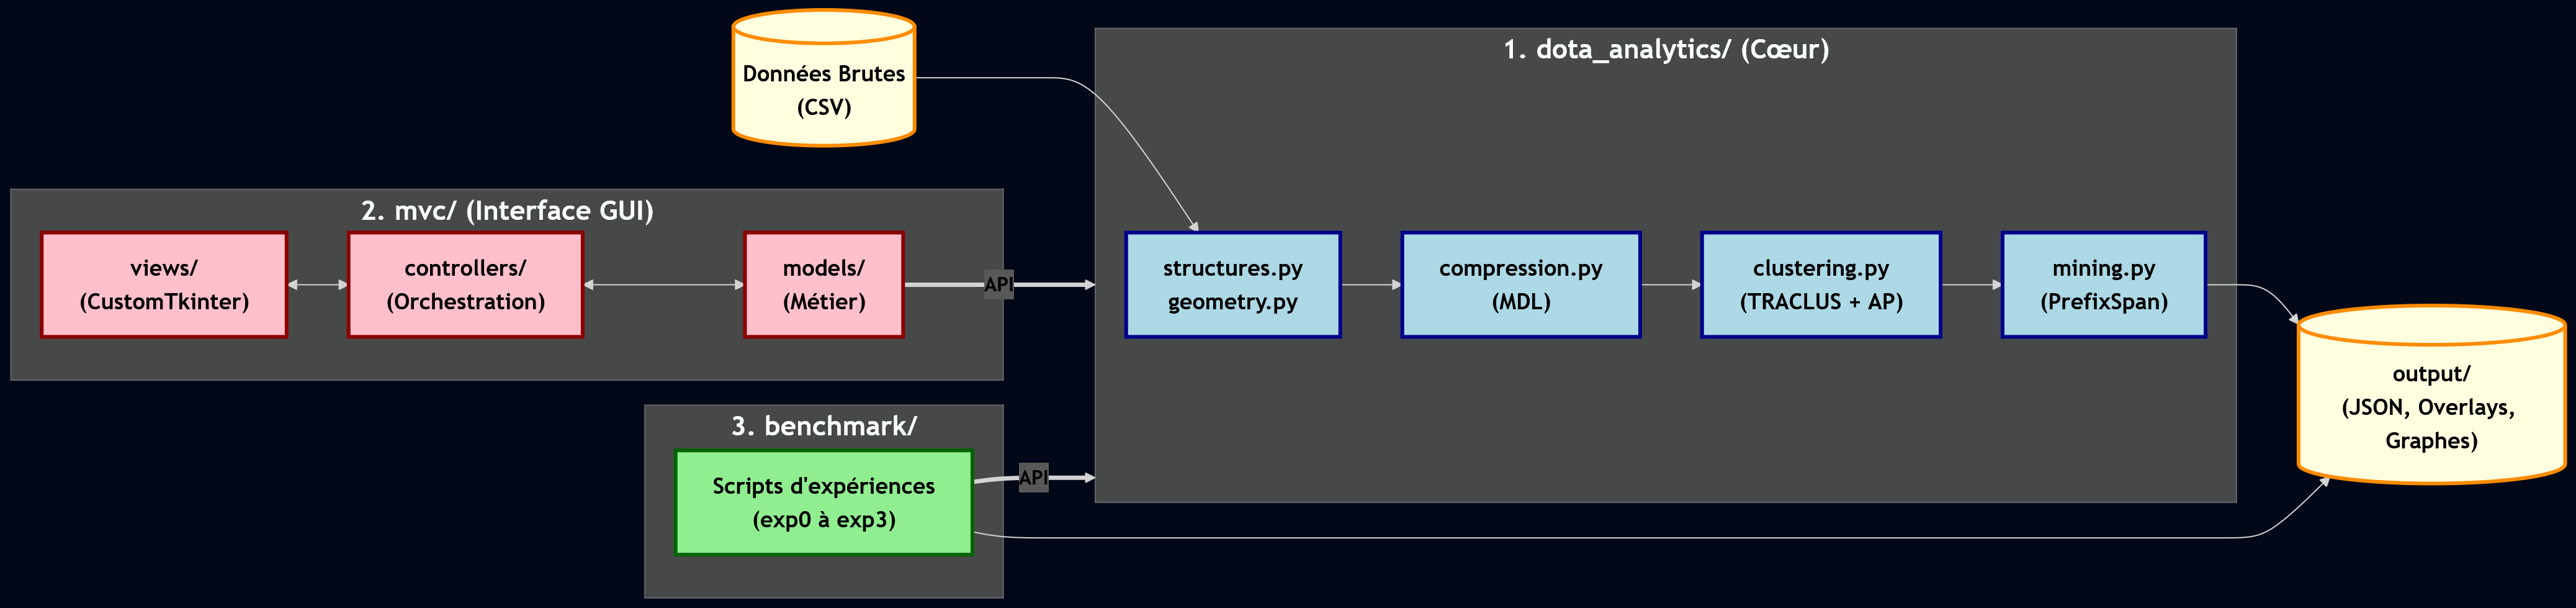
\includegraphics[width=1.0\textwidth, height=0.35\textheight, keepaspectratio]{img/diag_archi.png} 
    \caption{Architecture logicielle et flux de données du Dota 2 Trajectory Analyzer.}
    \label{fig:architecture}
\end{figure}

\subsection{Chaîne de Traitement}

Le projet s'organise selon un patron MVC : la bibliothèque \texttt{dota\_analytics} centralise les modèles et traitements réutilisables, tandis que le dossier \texttt{benchmark} fait office de laboratoire d'expérimentation, permettant de tester, calibrer et comparer chaque algorithme de manière isolée avant son intégration dans le pipeline final. Les données transitent séquentiellement au travers du pipeline décrit en Section 2.3 : les CSV bruts sont d'abord ingérés et compressés par \texttt{compression.py}, les segments résultants sont comparés via \texttt{metrics.py} (distance TRACLUS) et groupés par \texttt{clustering.py}, puis recodés par \texttt{recoding.py} et analysés par \texttt{mining.py}.

% ==========================================
% SECTION 6 : EXPÉRIMENTATIONS
% ==========================================
\section{Expérimentations}

Cette section présente l'ensemble de nos expérimentations, des cas d'utilisation concrets aux résultats quantitatifs détaillés.

\subsection{Cas d'Utilisation}

Afin d'illustrer concrètement les fonctionnalités décrites en Section 3, voici deux cas d'utilisation représentatifs de notre application.

\begin{figure}[H]
    \centering
    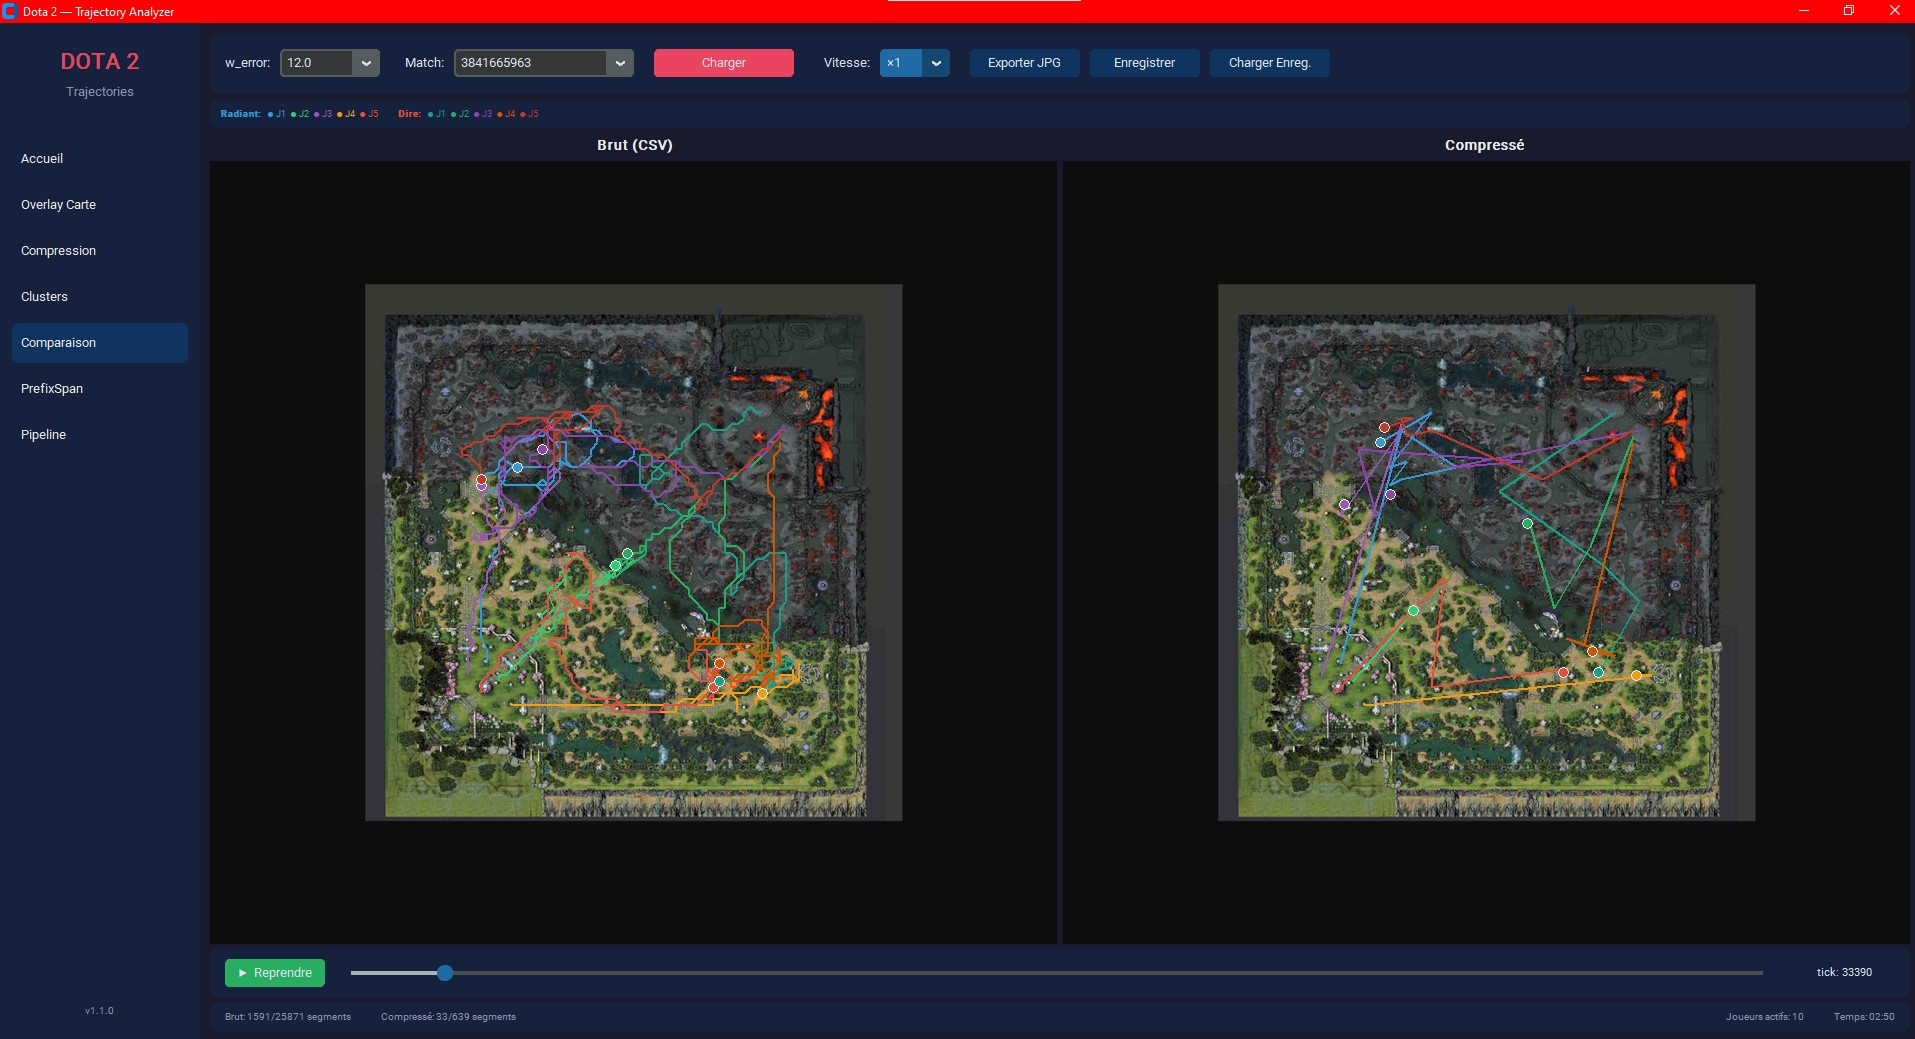
\includegraphics[width=0.9\textwidth, height=0.35\textheight, keepaspectratio]{img/CSV_vs_compressé.jpg} 
    \caption{Cas d'utilisation : Module de comparaison synchronisée Brut vs Compressé.}
    \label{fig:gui_comparison}
\end{figure}

La Figure \ref{fig:gui_comparison} montre le module de comparaison synchronisée, qui affiche deux cartes côte à côte permettant d'inspecter visuellement l'effet de la compression MDL sur une trajectoire.

\begin{figure}[H]
    \centering
    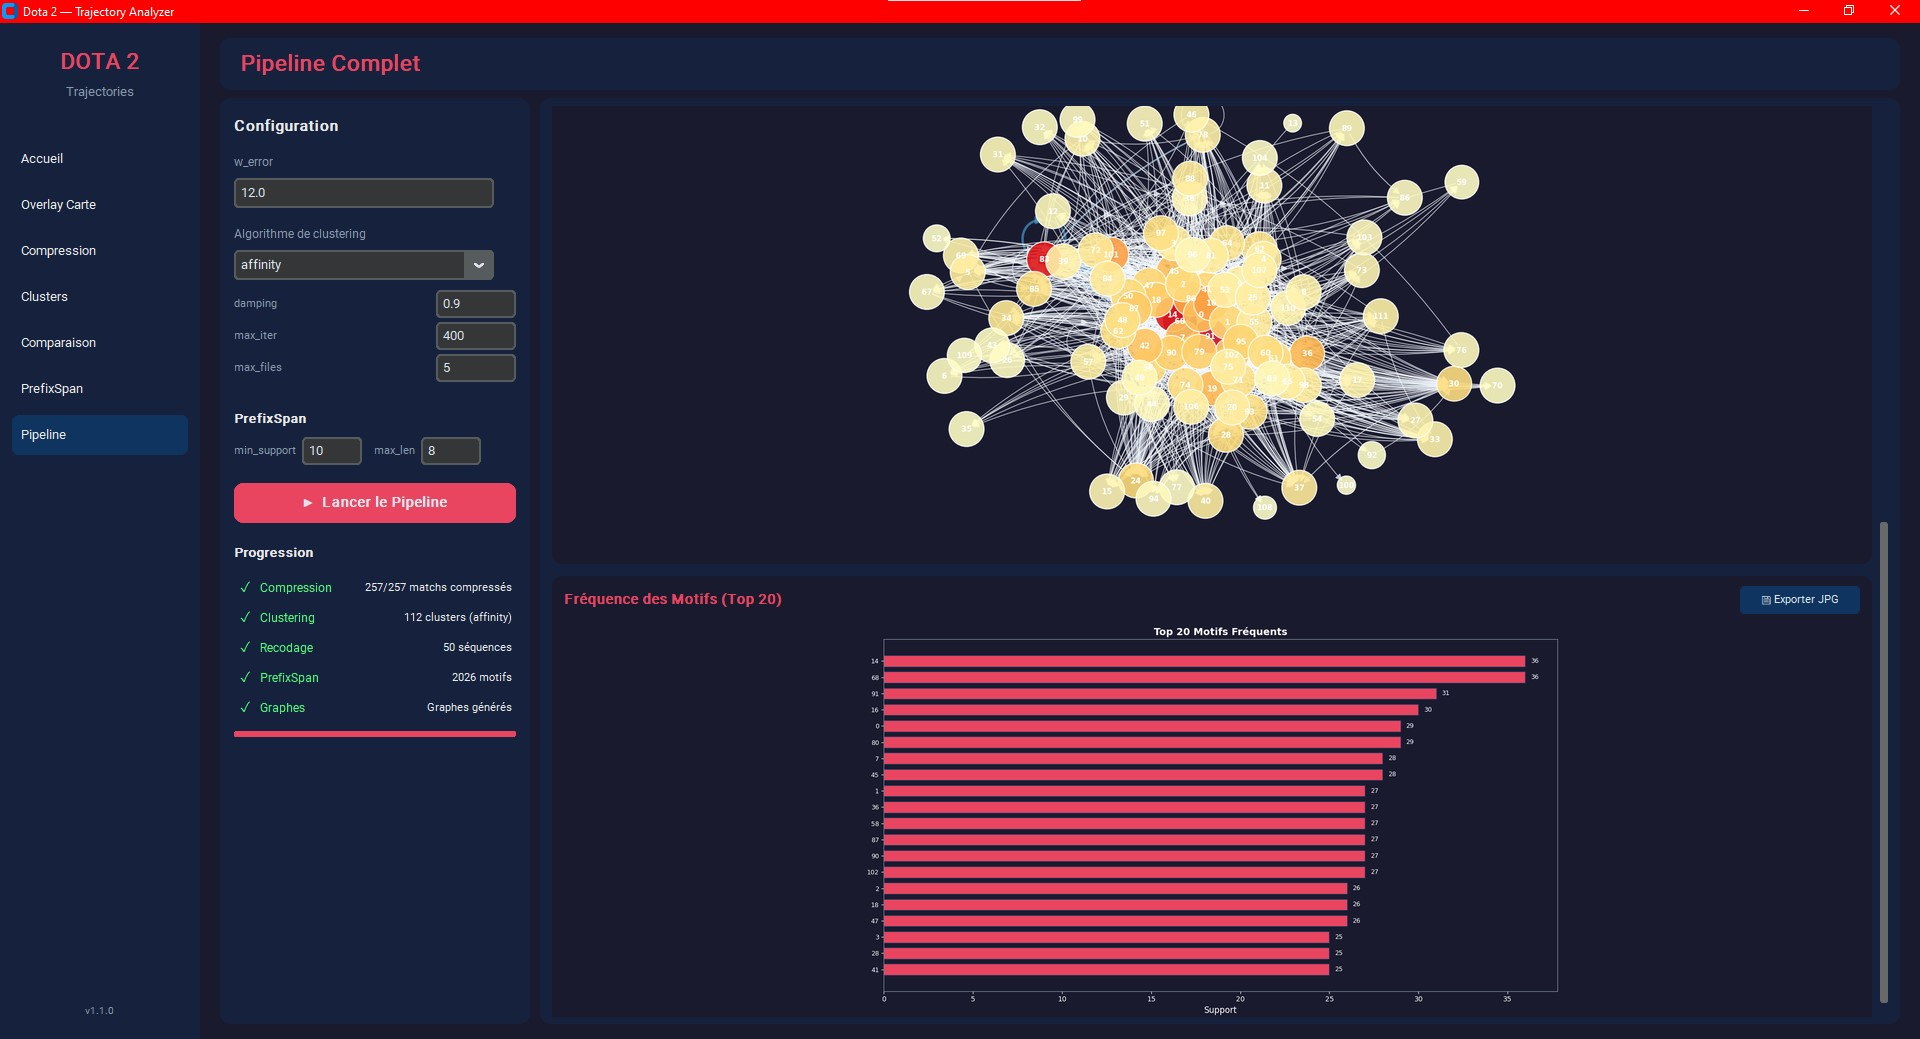
\includegraphics[width=0.9\textwidth, height=0.35\textheight, keepaspectratio]{img/pipeline_exemple1.jpg} 
    \caption{Cas d'utilisation : Exécution de l'orchestrateur de Pipeline avec restitution de l'analyse PrefixSpan.}
    \label{fig:gui_pipeline}
\end{figure}

La Figure \ref{fig:gui_pipeline} illustre l'orchestrateur end-to-end, qui automatise l'enchaînement complet du pipeline et restitue les résultats de l'analyse PrefixSpan.

% ------------------------------------------
% 6.2 : VALIDATION MDL
% ------------------------------------------
\subsection{Validation de la Compression par Seuil (MDL)}

Afin de valider rigoureusement notre implémentation de l'algorithme MDL, il était indispensable de dépasser la simple vérification visuelle pour adopter une démarche d'évaluation objective et quantitative.

\subsubsection{Vérification du Fonctionnement}
Pour évaluer la qualité de la compression sur un large volume de données, nous avons mesuré l'erreur spatiale (RMSE) et le taux de compression sur un ensemble représentatif de trajectoires.

\begin{figure}[H]
  \centering
  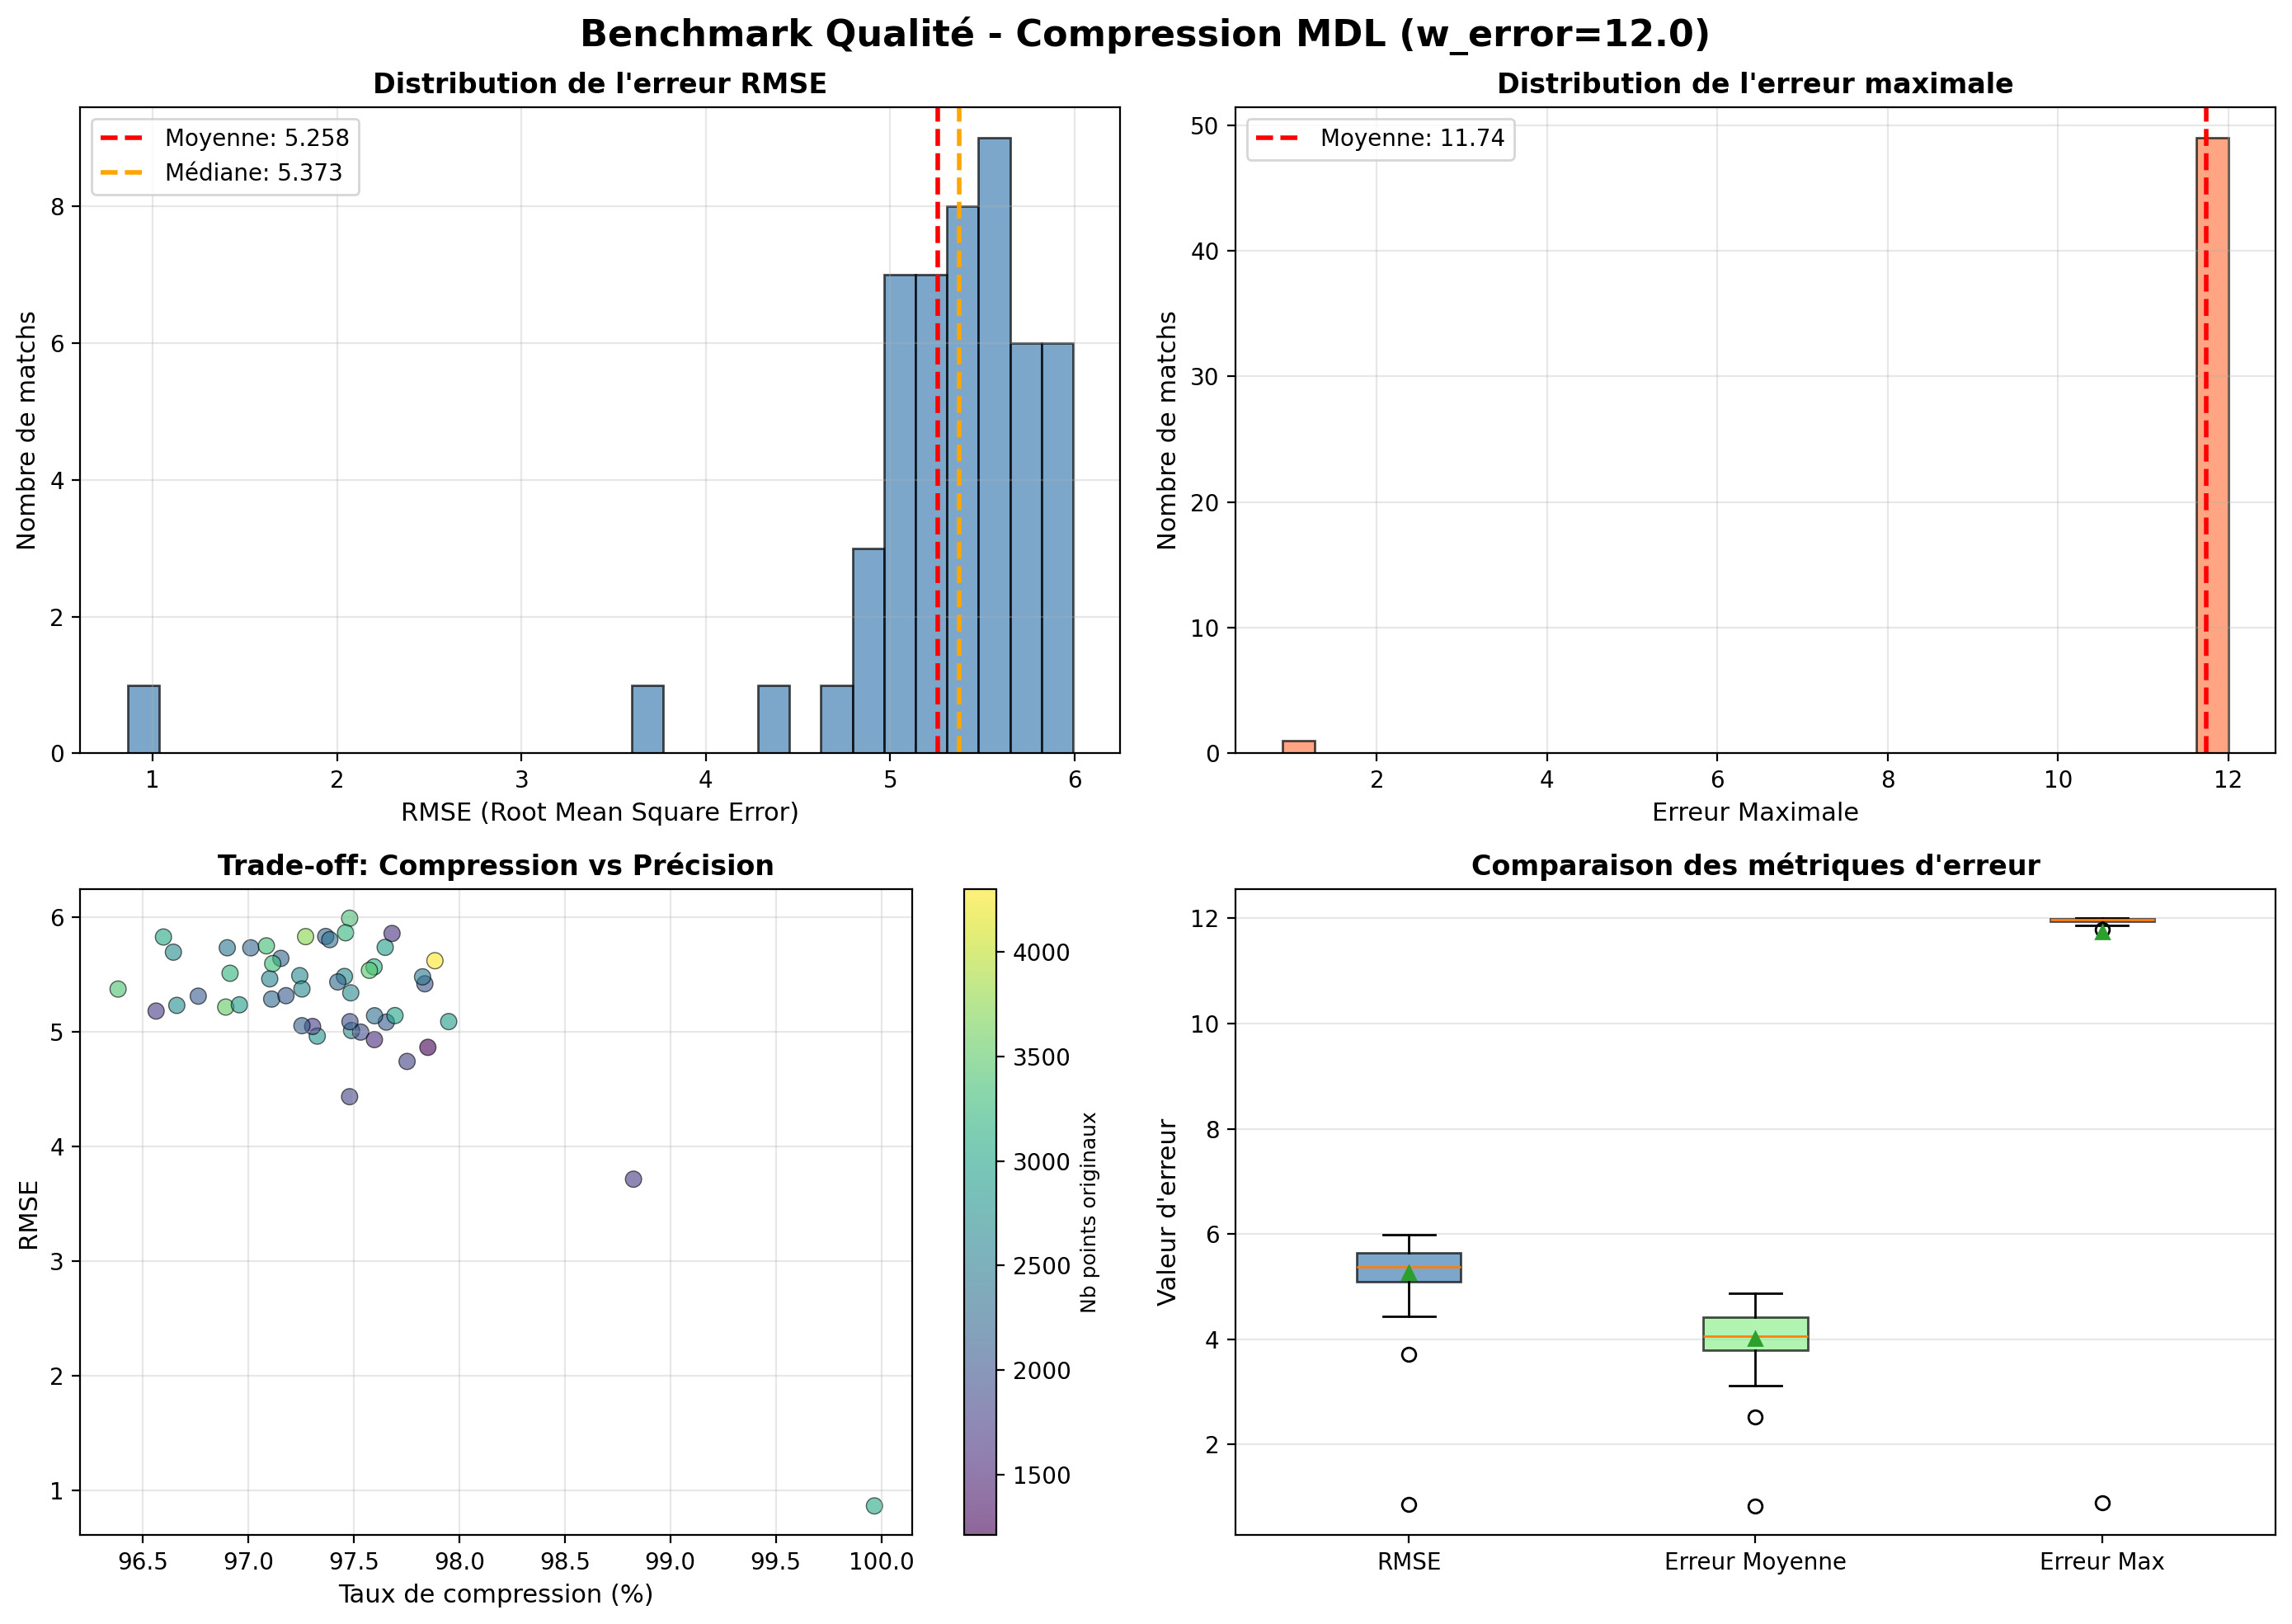
\includegraphics[width=\textwidth, height=0.3\textheight, keepaspectratio]{img/benchmark_quality.jpg}
  \caption{Distribution de l'erreur maximale et compromis Compression/Précision.}
  \label{fig:benchmark_quality}
\end{figure}

L'analyse de la Figure \ref{fig:benchmark_quality} met en évidence deux observations importantes :
\begin{itemize}
    \item \textbf{Plafonnement de l'Erreur Maximale :} La distribution montre que l'erreur maximale est strictement contenue juste sous la barre des 12 unités. Cela confirme que l'approche "Greedy" respecte notre paramètre $w_{error}=12$.
    \item \textbf{Trade-off Compression vs Précision :} On observe une concentration optimale entre 96,5\% et 98,0\% de taux de compression, pour un RMSE contenu.
\end{itemize}

\subsubsection{Invariance au Bruit et Stabilité Structurelle}
Pour tester la robustesse face aux comportements erratiques, nous avons injecté un bruit gaussien artificiel sur les trajectoires.

\begin{figure}[H]
  \centering
  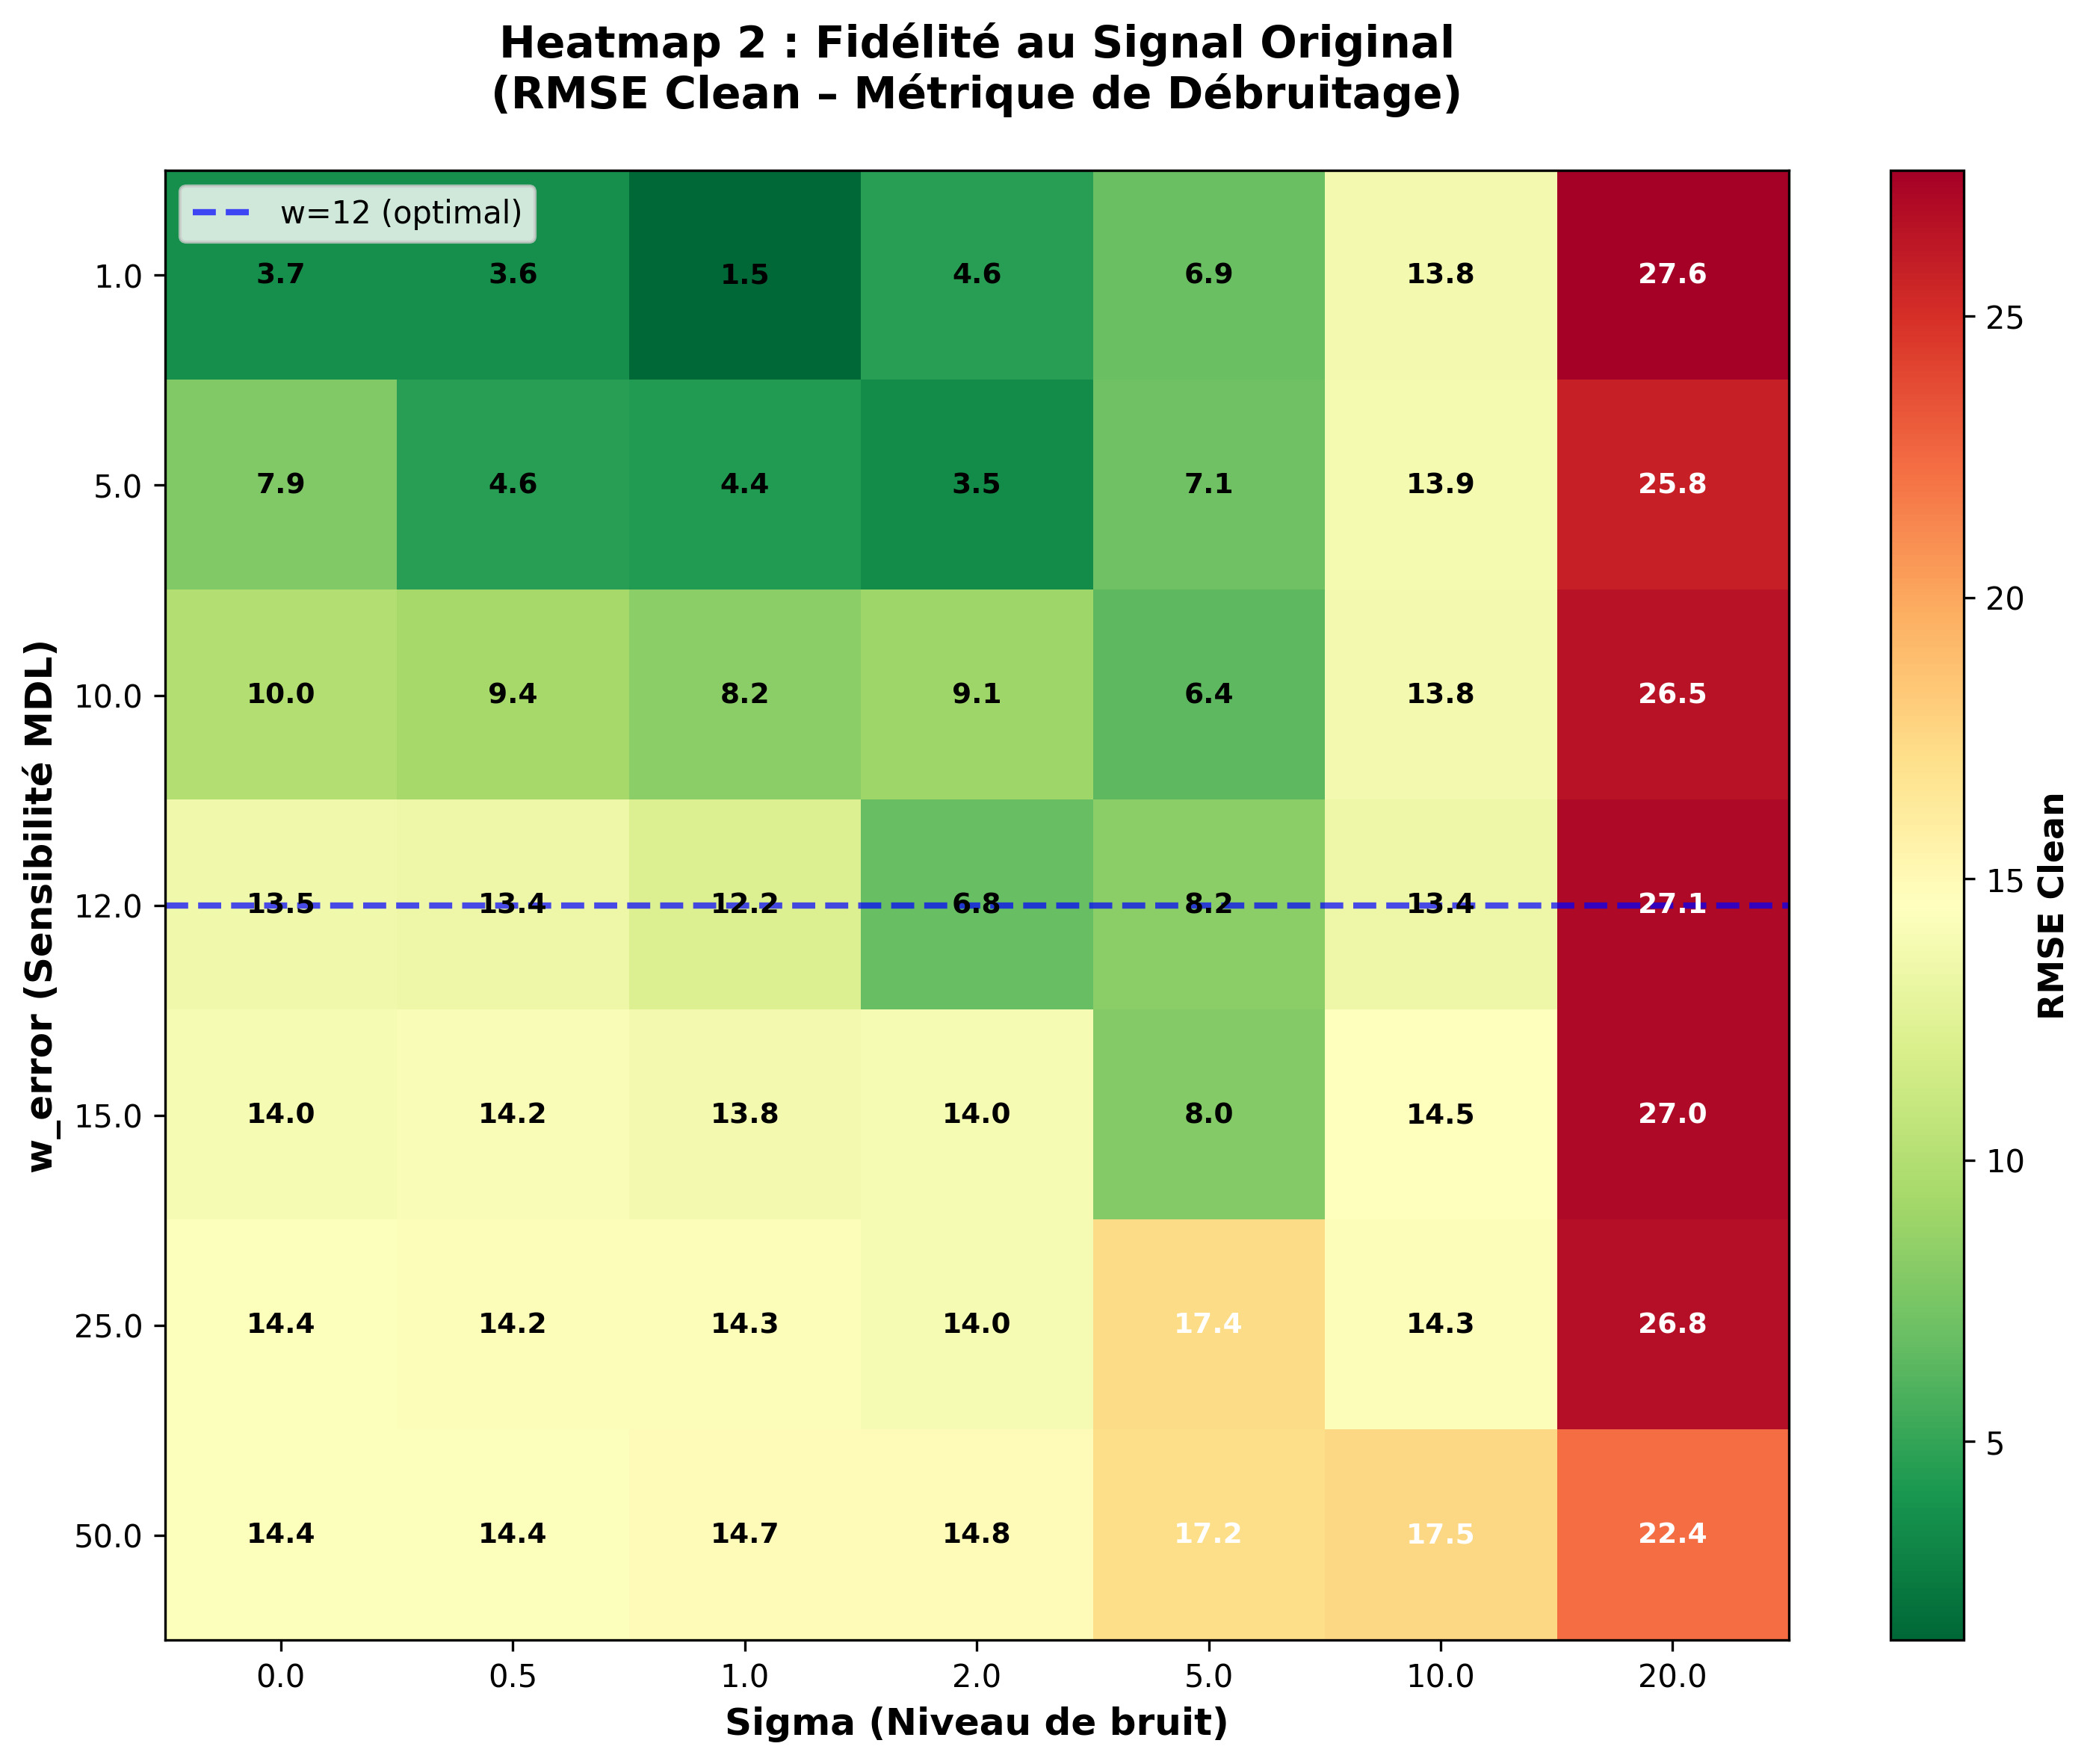
\includegraphics[width=\textwidth, height=0.3\textheight, keepaspectratio]{img/heatmap_fidelite.jpg}
  \caption{Étude de stabilité structurelle face au bruit gaussien : Évolution du nombre de segments et du RMSE.}
  \label{fig:heatmaps_bruit}
\end{figure}

Comme illustré par la Figure \ref{fig:heatmaps_bruit}, l'étude révèle que pour $w_{error} = 12.0$, le nombre de segments générés reste parfaitement stable pour des niveaux de bruit $\sigma \le 2.0$. L'algorithme absorbe efficacement les petites perturbations sans modifier la forme globale de la trajectoire.

\subsubsection{Validation Visuelle de la Robustesse}
\begin{figure}[H]
  \centering
  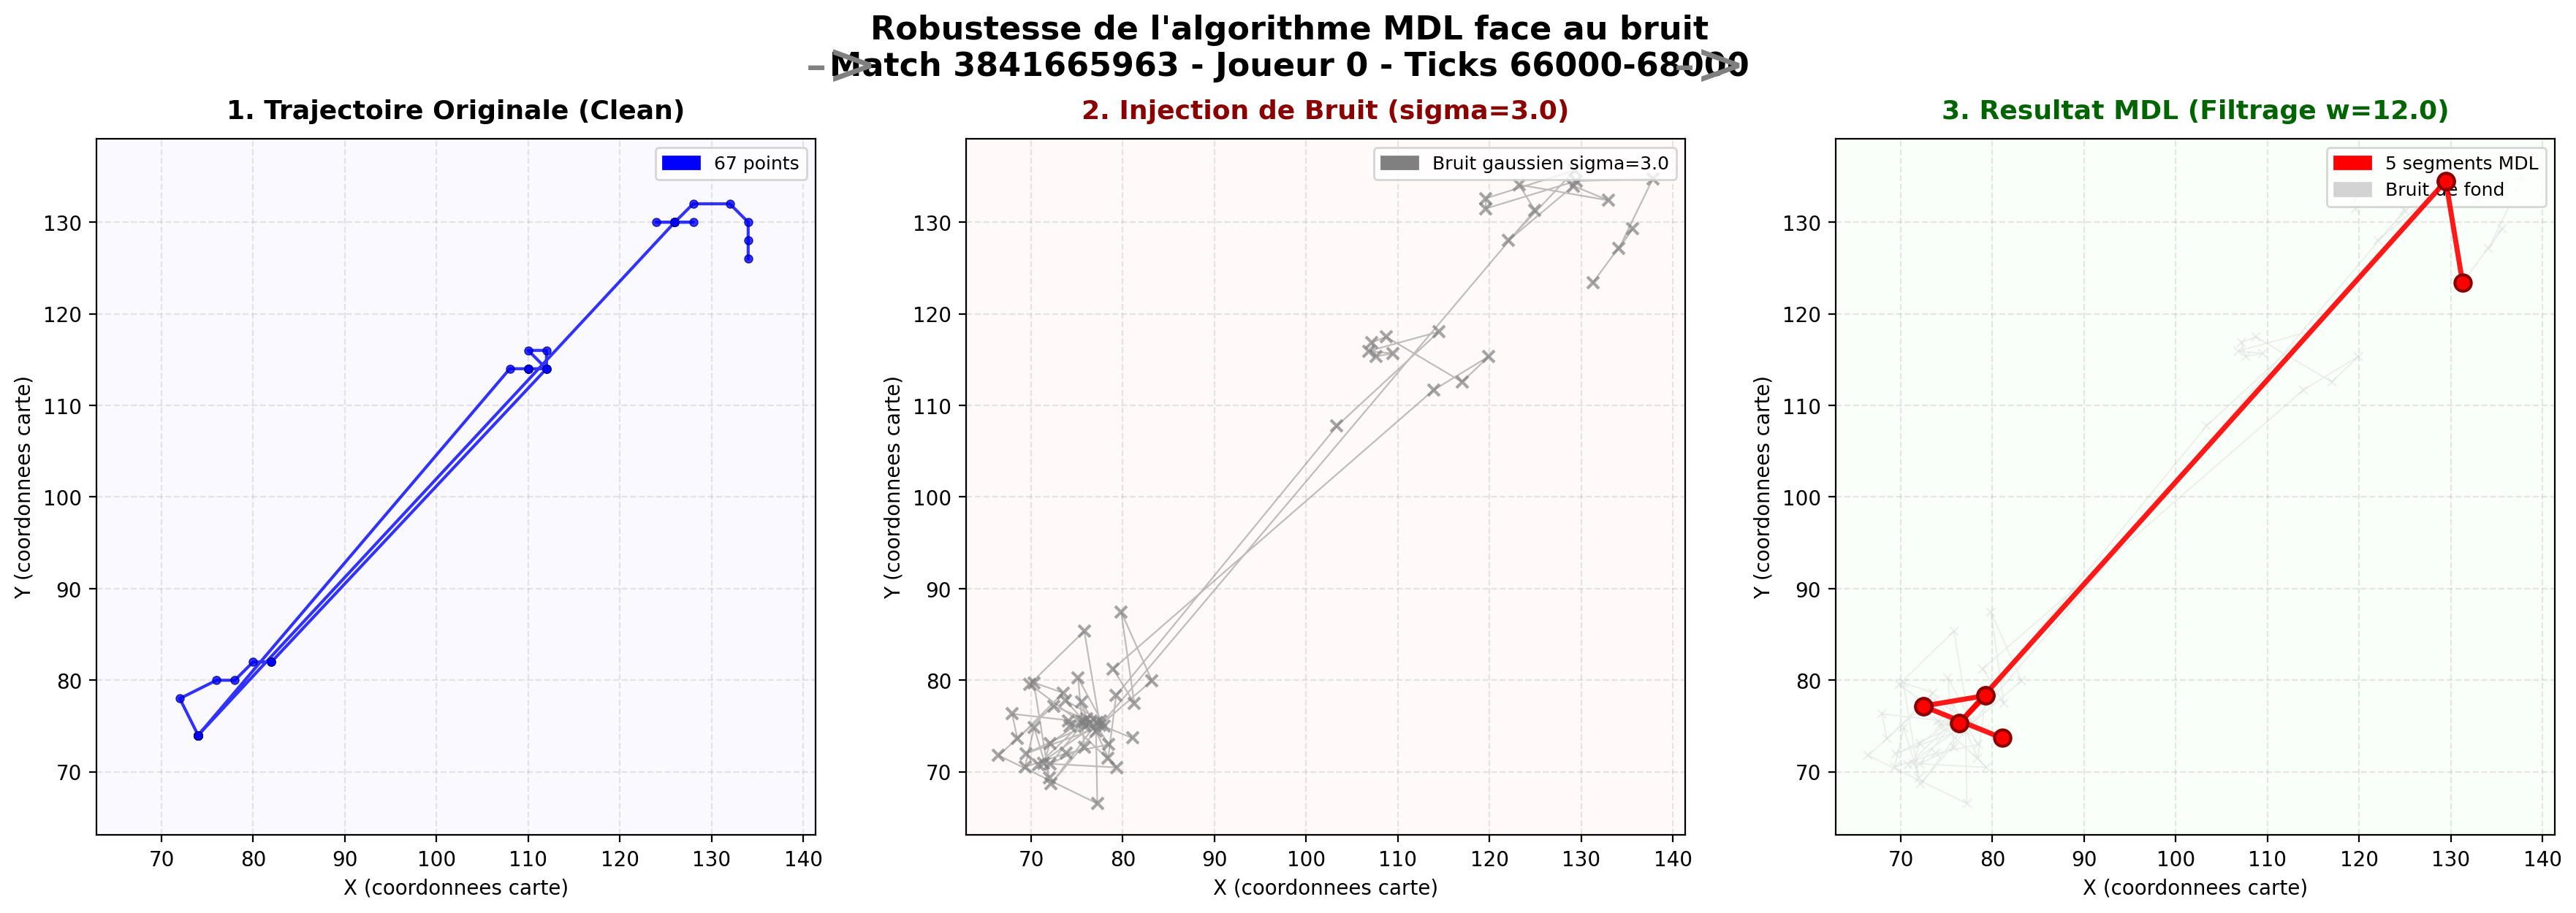
\includegraphics[width=\textwidth, height=0.3\textheight, keepaspectratio]{img/triptych_w12_sigma3.jpg}
  \caption{Reconstruction d'une trajectoire à partir de données hautement bruitées.}
  \label{fig:visu_robustesse}
\end{figure}

Comme le démontre la Figure \ref{fig:visu_robustesse}, face à un nuage chaotique simulant de multiples micro-clics, la compression MDL parvient à extraire des segments nets passant par le centre du nuage de points, conservant ainsi la forme globale du déplacement.

\subsubsection{Évaluation Comparative avec les Méthodes Standards (Baseline)}
Nous comparons MDL à l'échantillonnage uniforme et à l'algorithme de Douglas-Peucker \cite{douglas1973} à \textbf{taux de compression égal} ($\approx 95\%$), en ajustant les paramètres de chaque méthode pour atteindre ce taux.

\begin{figure}[H]
  \centering
  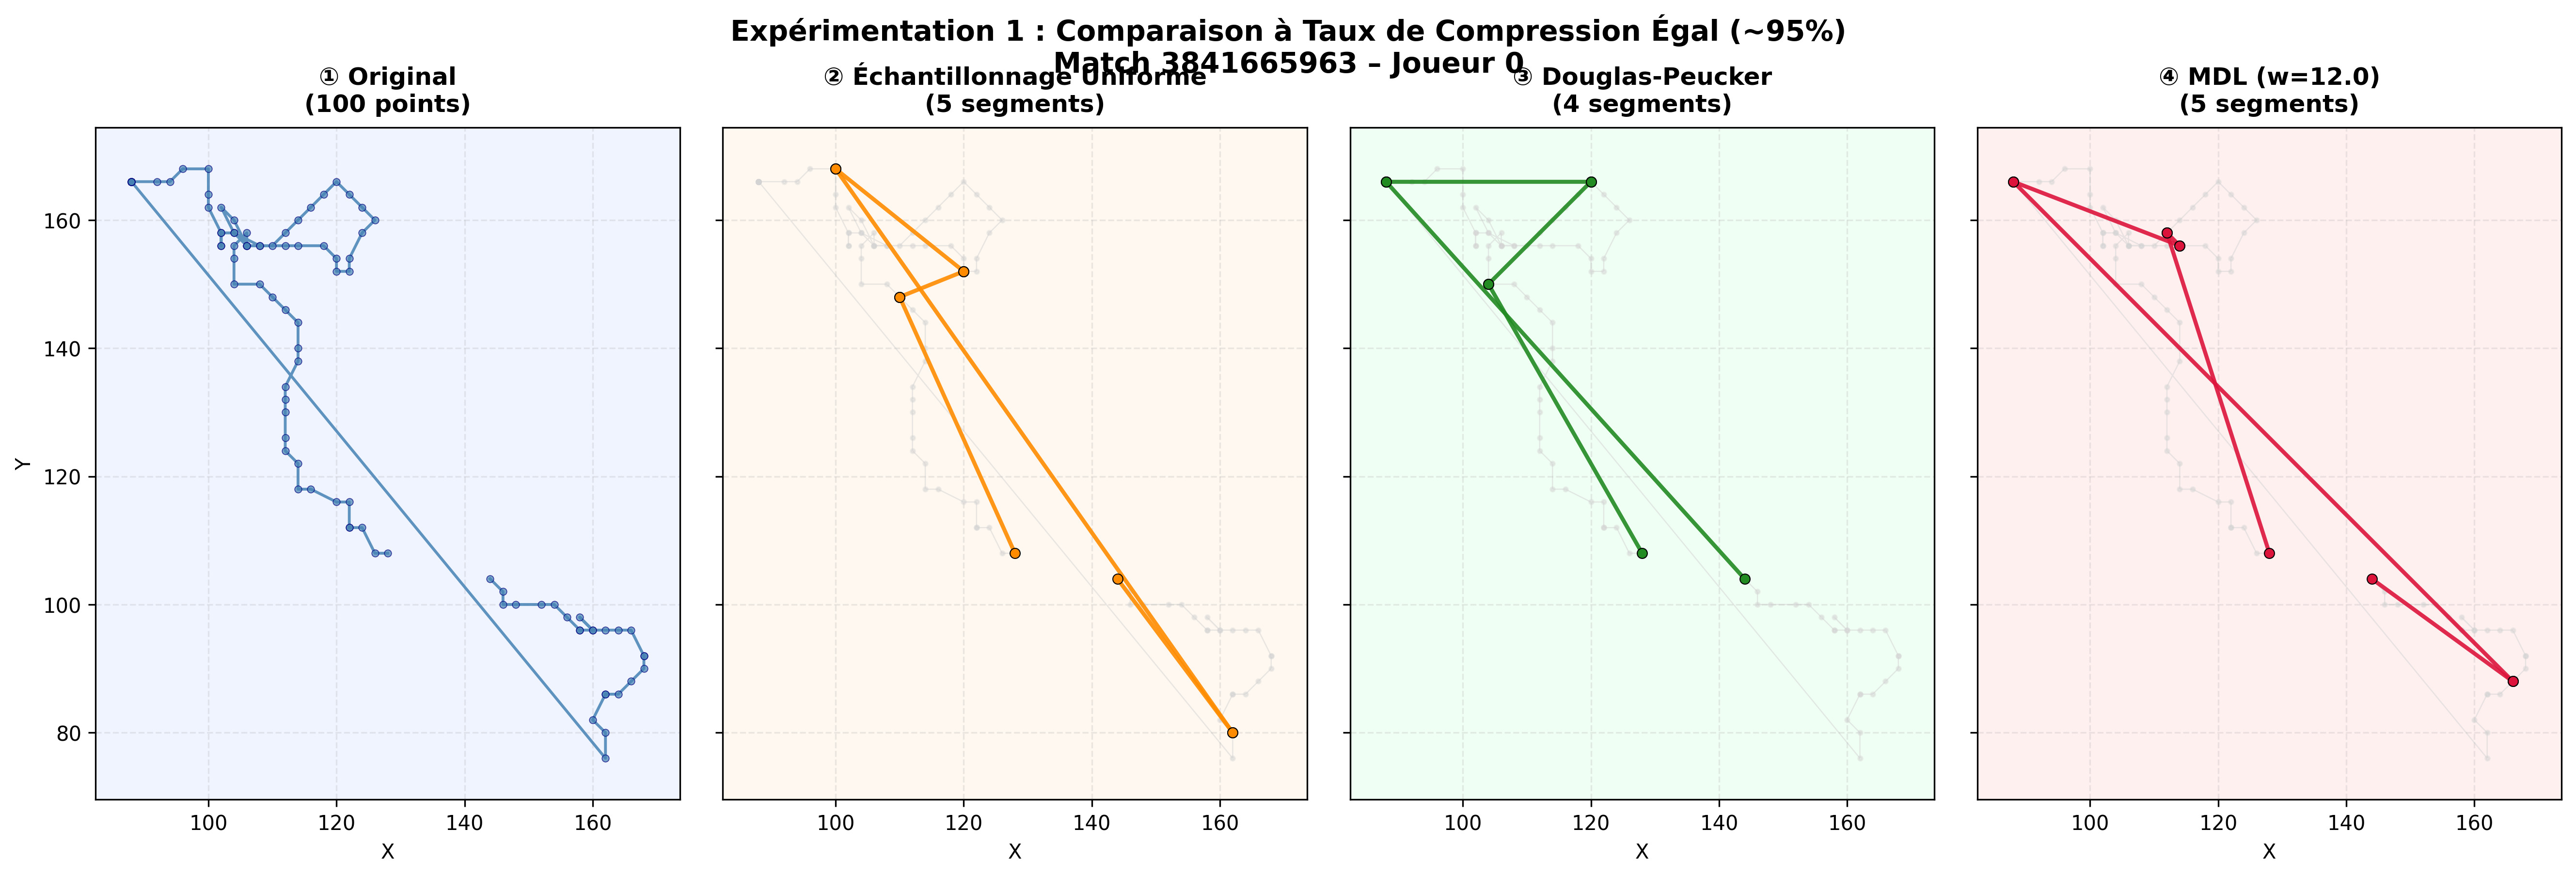
\includegraphics[width=\textwidth, height=0.28\textheight, keepaspectratio]{img/baseline_comparison.jpg}
  \caption{Comparaison visuelle des algorithmes de compression face à une trajectoire réelle.}
  \label{fig:baseline_comparison}
\end{figure}

Sur la Figure \ref{fig:baseline_comparison}, on observe visuellement que l'échantillonnage Uniforme crée des trajectoires erratiques, tandis que Douglas-Peucker se laisse piéger par les \textit{outliers}. 

\begin{figure}[H]
    \centering
    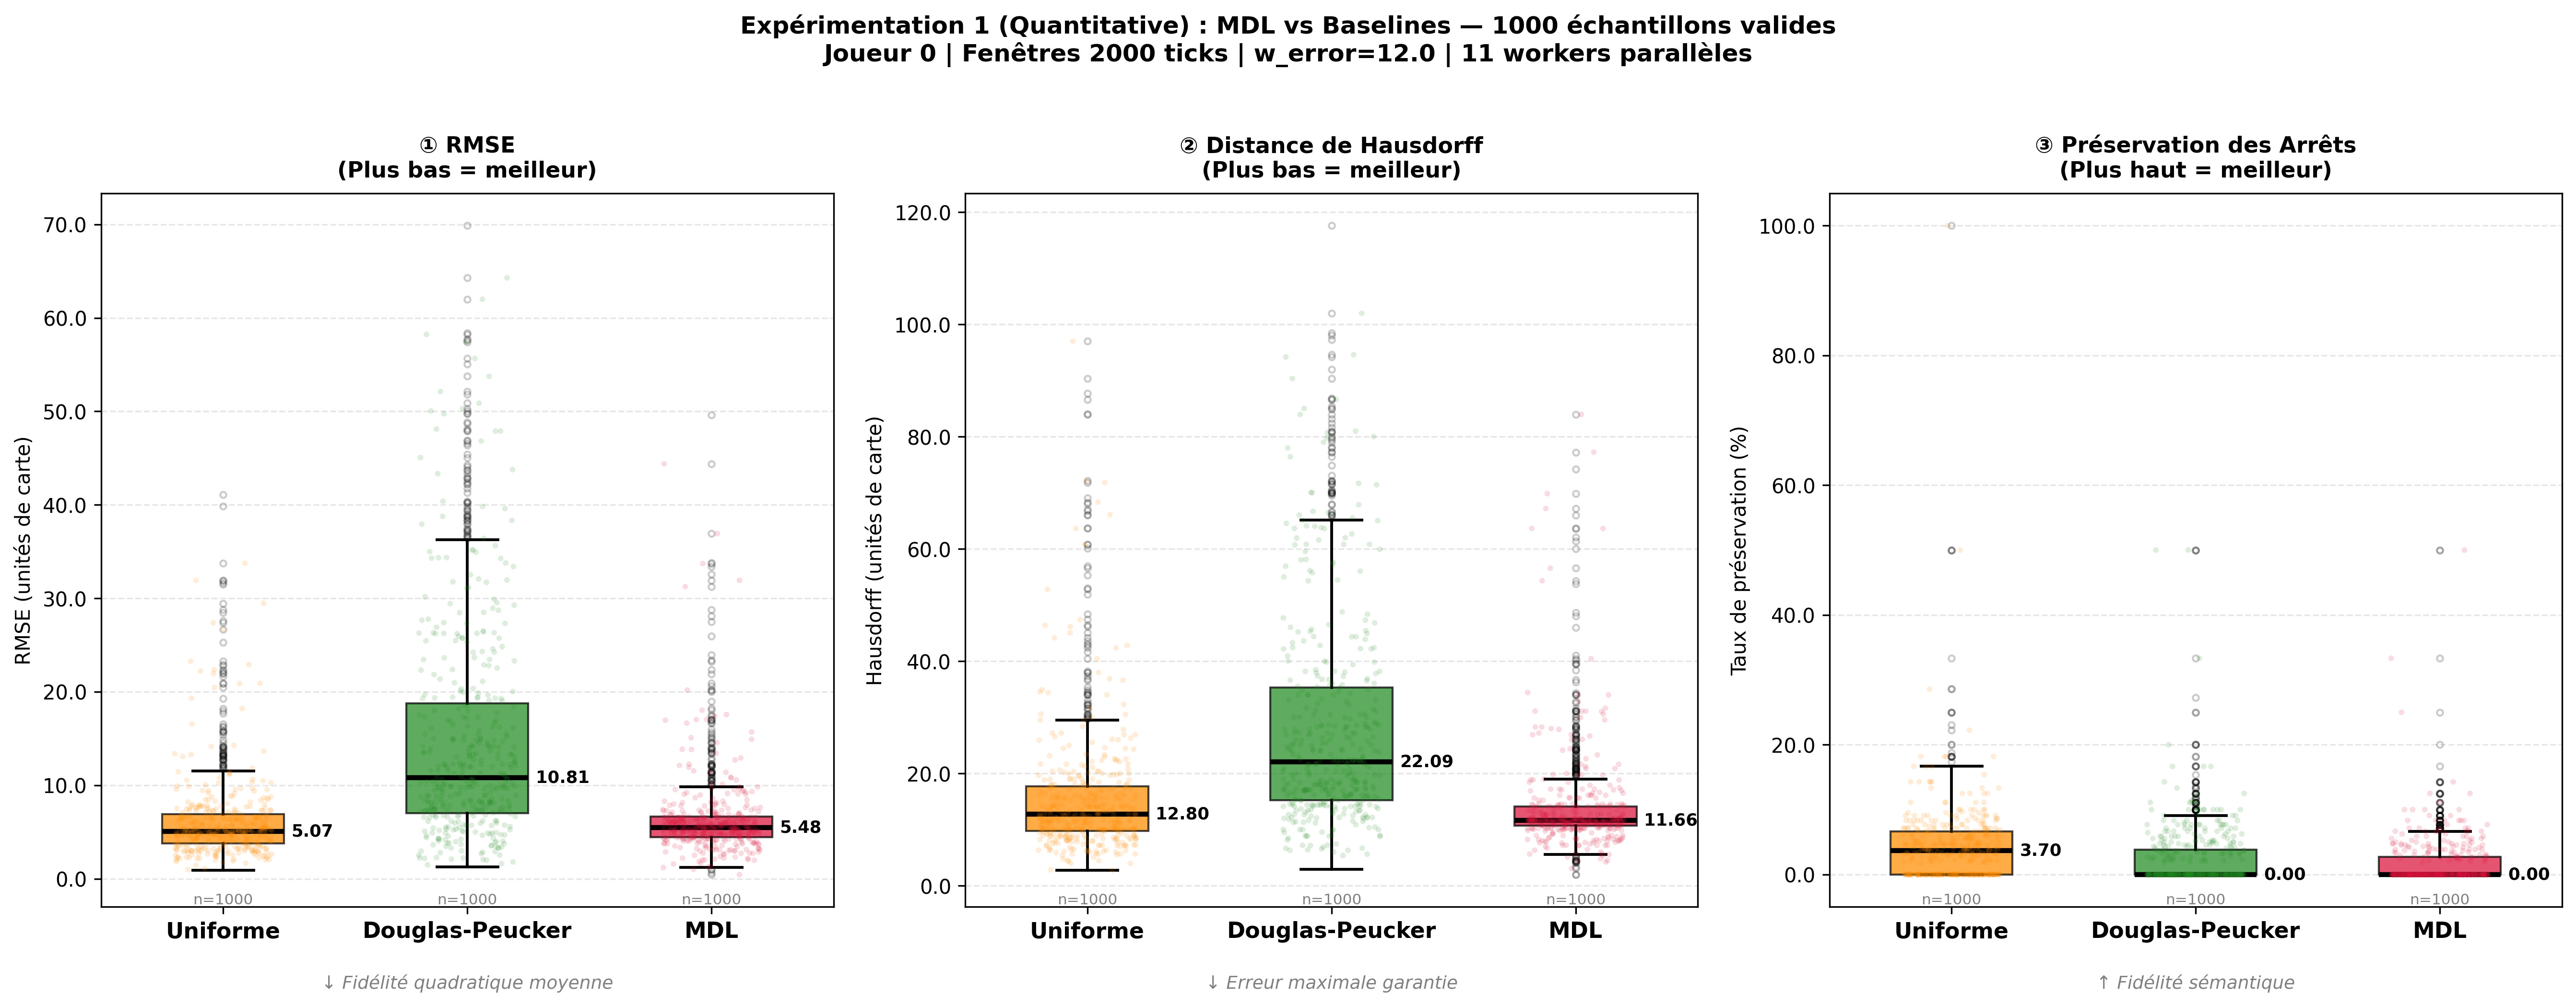
\includegraphics[width=0.8\textwidth, height=0.28\textheight, keepaspectratio]{img/baseline_maths_boxplots.jpg}
    \caption{Analyse statistique (Boxplots) des algorithmes sur 1000 trajectoires de joueurs issues des matchs disponibles.}
    \label{fig:baseline_maths}
\end{figure}

L'analyse statistique détaillée (Figure \ref{fig:baseline_maths}) révèle les différences suivantes :
\begin{itemize}
    \item \textbf{Fidélité Quadratique Moyenne (RMSE) :} L'échantillonnage uniforme (médiane à 5.07) et MDL (5.48) obtiennent des résultats nettement meilleurs que Douglas-Peucker (10.81). 
    \item \textbf{Erreur Maximale (Distance de Hausdorff) :} MDL obtient la meilleure fidélité géométrique (médiane à 11.66, contre 12.80 pour l'uniforme et 22.09 pour DP), ce qui limite l'écart maximal entre la trajectoire originale et la trajectoire compressée.
    \item \textbf{Information temporelle :} Ces trois méthodes, étant purement spatiales, ne préservent pas l'information de durée de pause aux points intermédiaires supprimés.
\end{itemize}

Le Tableau \ref{tab:baseline} résume ces résultats de manière synthétique.

\begin{table}[H]
\centering
\caption{Récapitulatif de la comparaison des algorithmes de compression (à taux de compression $\approx 95\%$).}
\label{tab:baseline}
\begin{tabular}{lccc}
\toprule
\textbf{Métrique} & \textbf{Uniforme} & \textbf{Douglas-Peucker} & \textbf{MDL} \\
\midrule
RMSE (médiane) & 5.07 & 10.81 & 5.48 \\
Hausdorff (médiane) & 12.80 & 22.09 & \textbf{11.66} \\
Préservation temporelle & Non & Non & Non \\
\bottomrule
\end{tabular}
\end{table}

\subsubsection{Évaluation de la Complexité Computationnelle}
\begin{figure}[H]
  \centering
  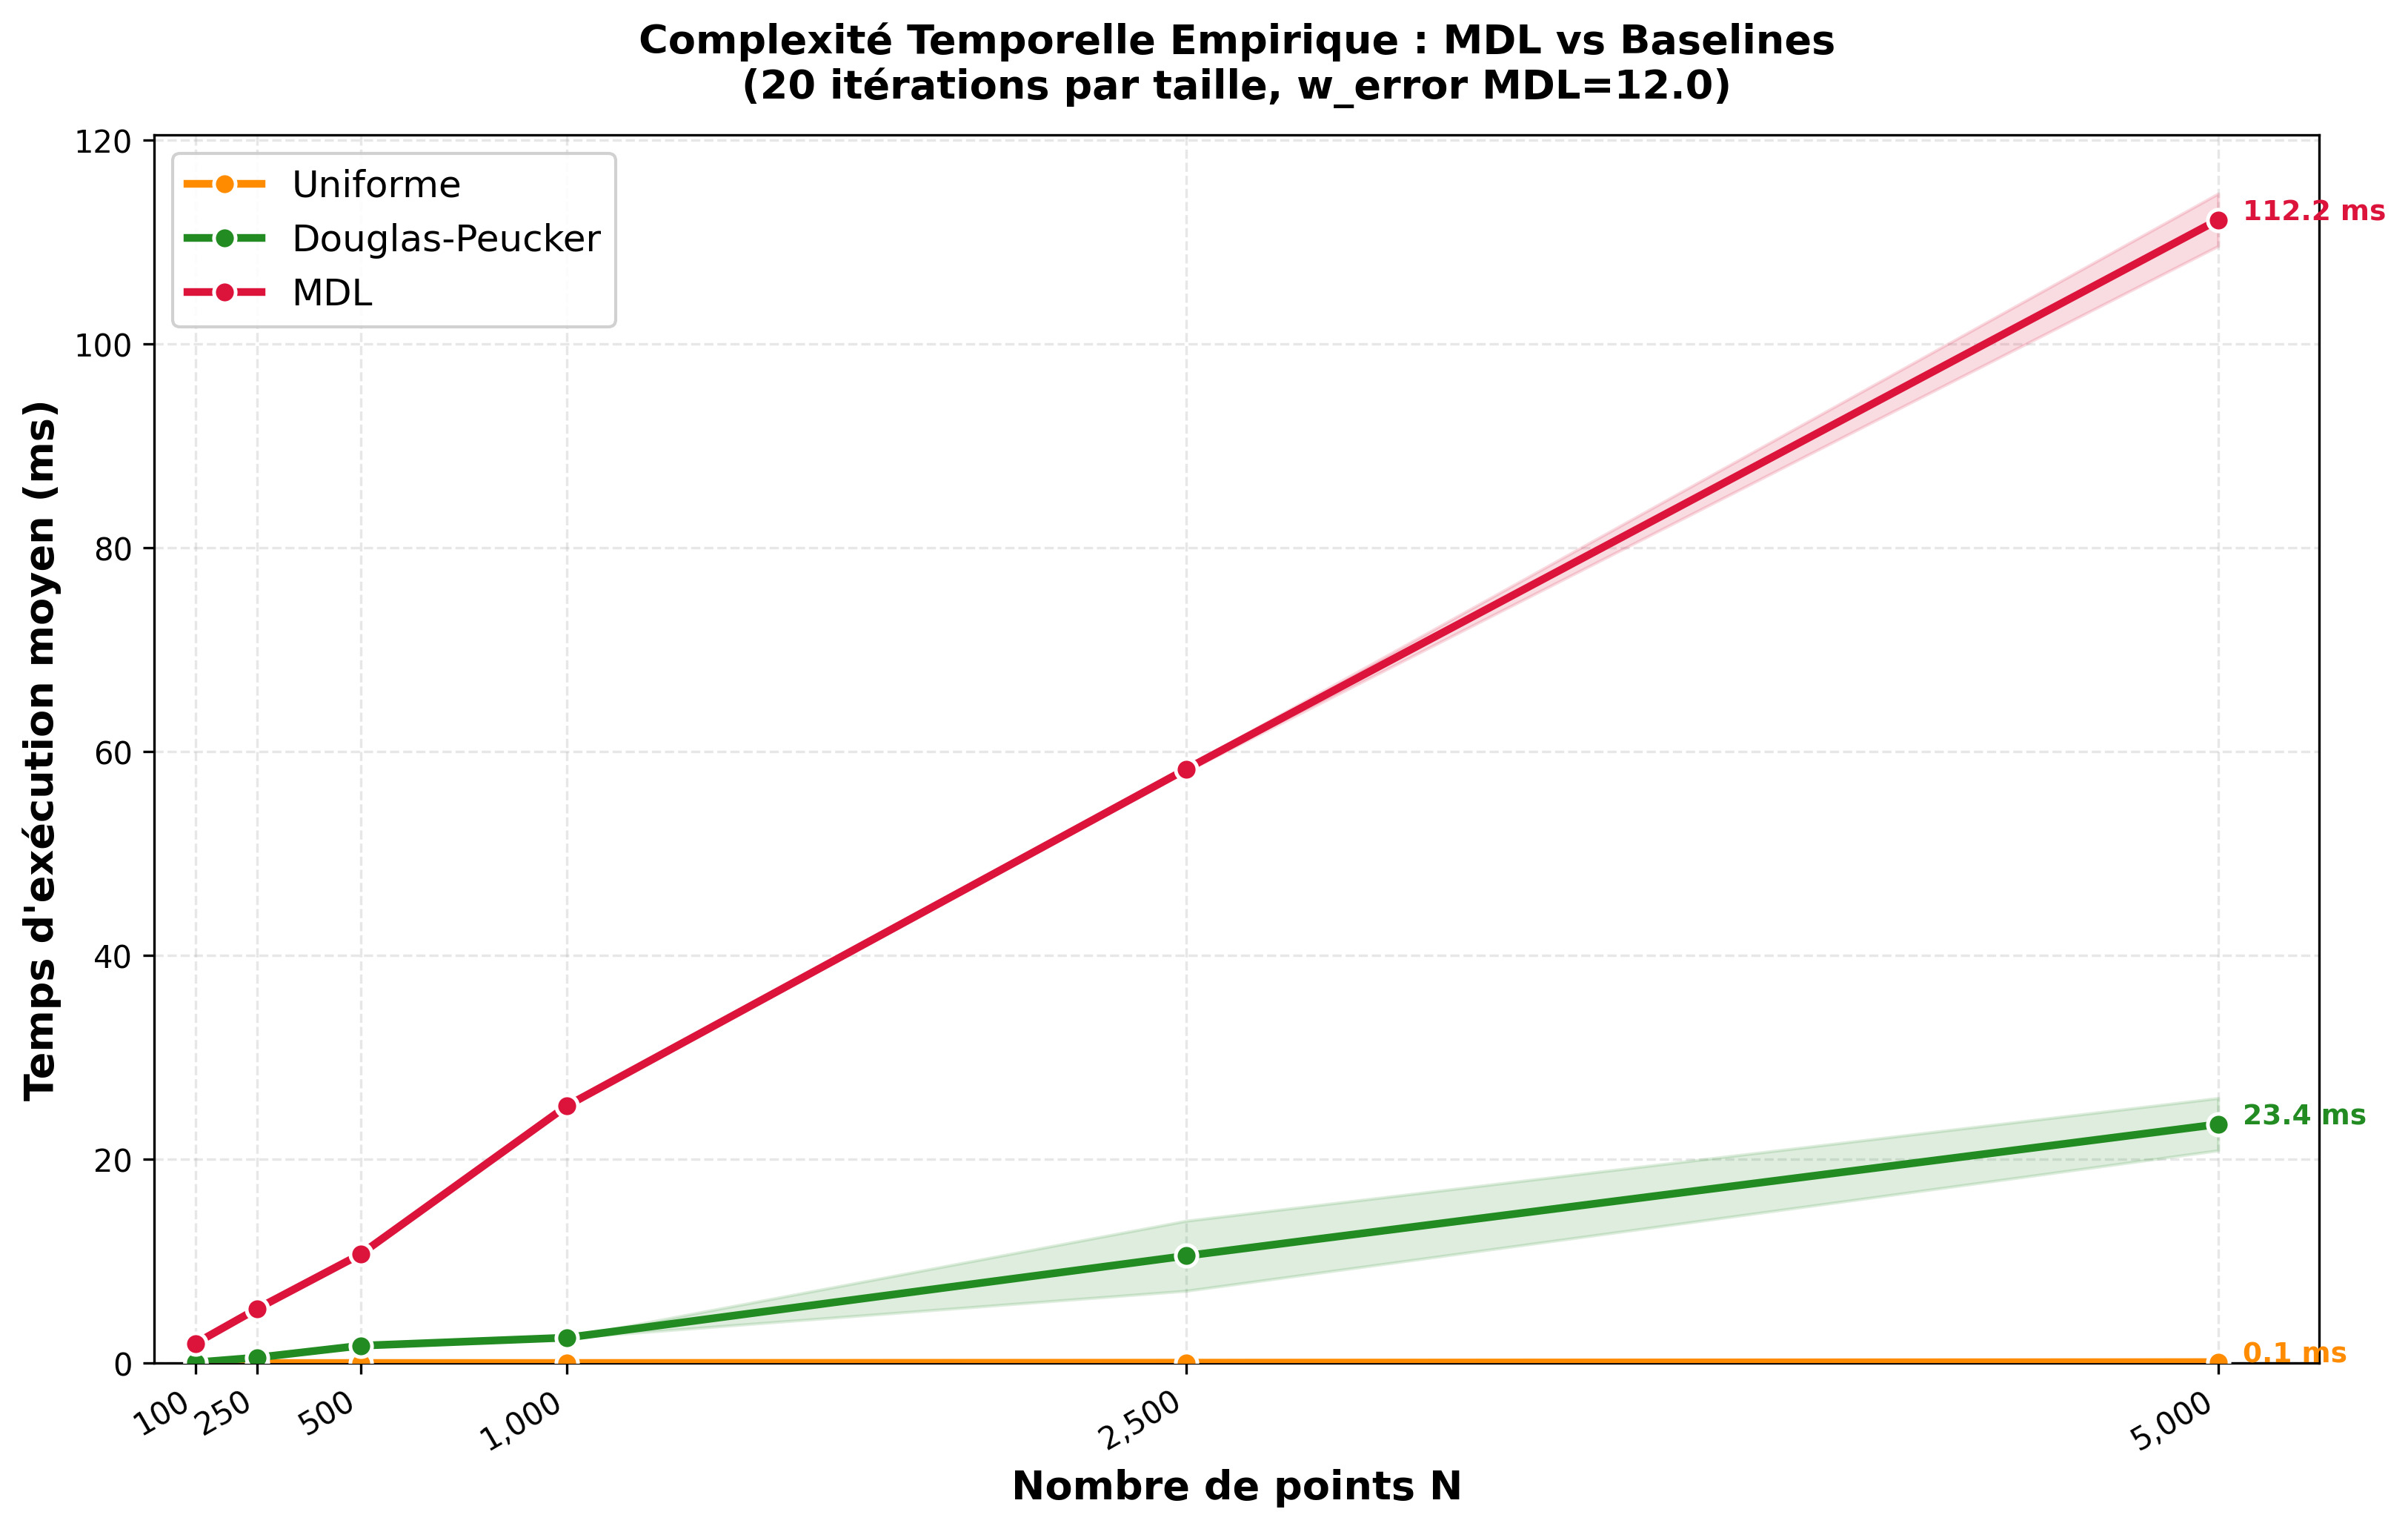
\includegraphics[width=0.8\textwidth, height=0.3\textheight, keepaspectratio]{img/time_complexity_plot.jpg}
  \caption{Benchmark de complexité temporelle empirique ($w_{error}=12.0$).}
  \label{fig:time_complexity}
\end{figure}

D'après la Figure \ref{fig:time_complexity}, l'implémentation MDL affiche un coût computationnel de l'ordre de $\mathcal{O}(N^2)$ dans le pire cas, atteignant 7,19 secondes pour 5000 points. En pratique, le \textit{break} anticipé dans la boucle interne réduit ce coût moyen, ce qui explique la courbe empirique située entre $\mathcal{O}(N^{1.5})$ et $\mathcal{O}(N^2)$. Un temps de traitement \textit{offline} de 7 secondes par demi-heure de jeu reste acceptable pour un usage non temps-réel. 

\subsubsection{Analyse de Sensibilité : Justification du paramètre $w_{error}$}

Pour justifier empiriquement le choix de notre tolérance d'erreur, nous avons fait varier $w_{error}$ de 0 à 50 et mesuré son impact sur l'ensemble de la chaîne de traitement. 

\begin{figure}[H]
    \centering
    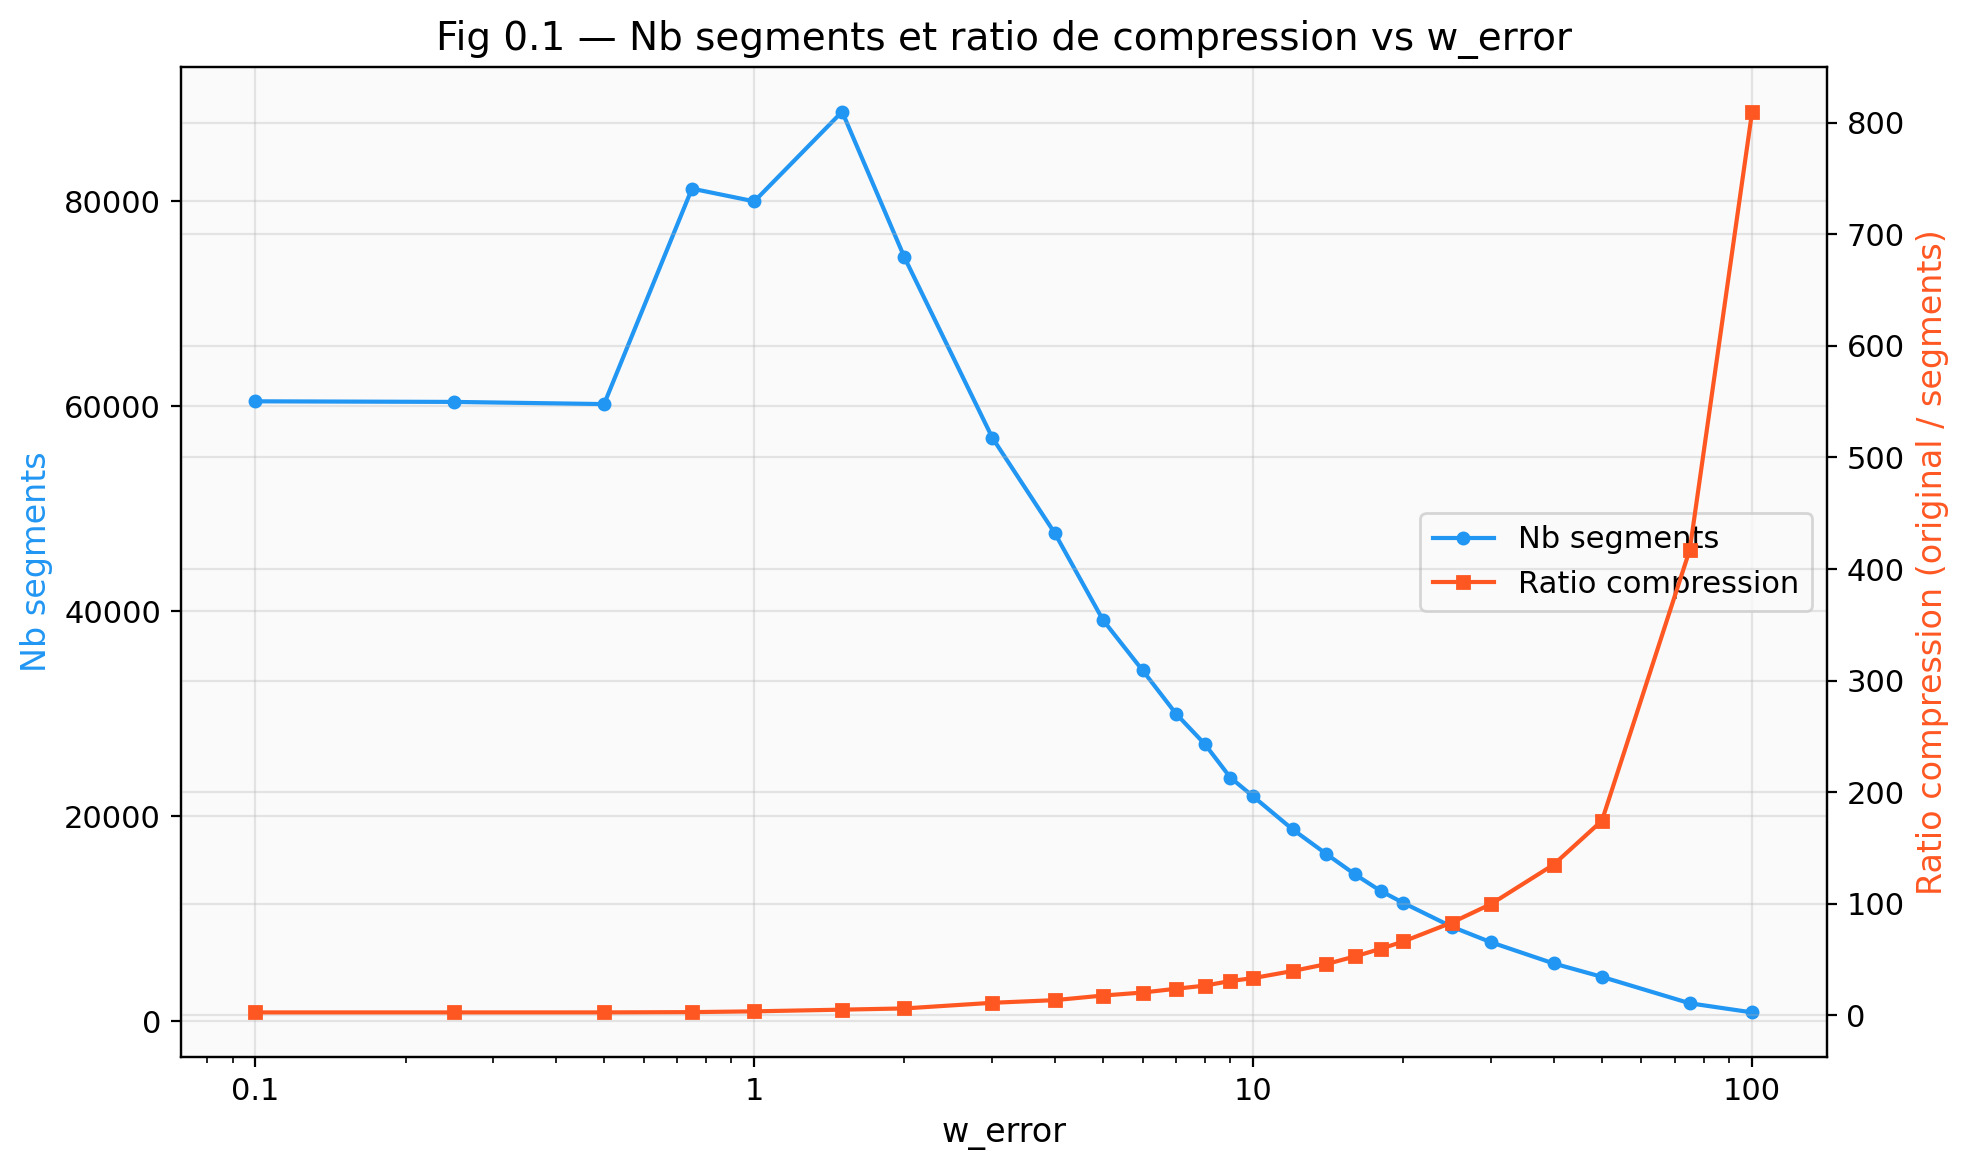
\includegraphics[width=0.9\textwidth, height=0.28\textheight, keepaspectratio]{img/fig0_1_segments_compression.jpg}
    \caption{Évolution du nombre de segments et du ratio de compression en fonction de $w_{error}$.}
    \label{fig:compression_ratio}
\end{figure}

La Figure \ref{fig:compression_ratio} montre qu'au-delà de $w_{error} = 12$, le gain en compression marginal plafonne autour de 96\% et ne justifie plus la perte d'information géométrique. 

\begin{figure}[H]
    \centering
    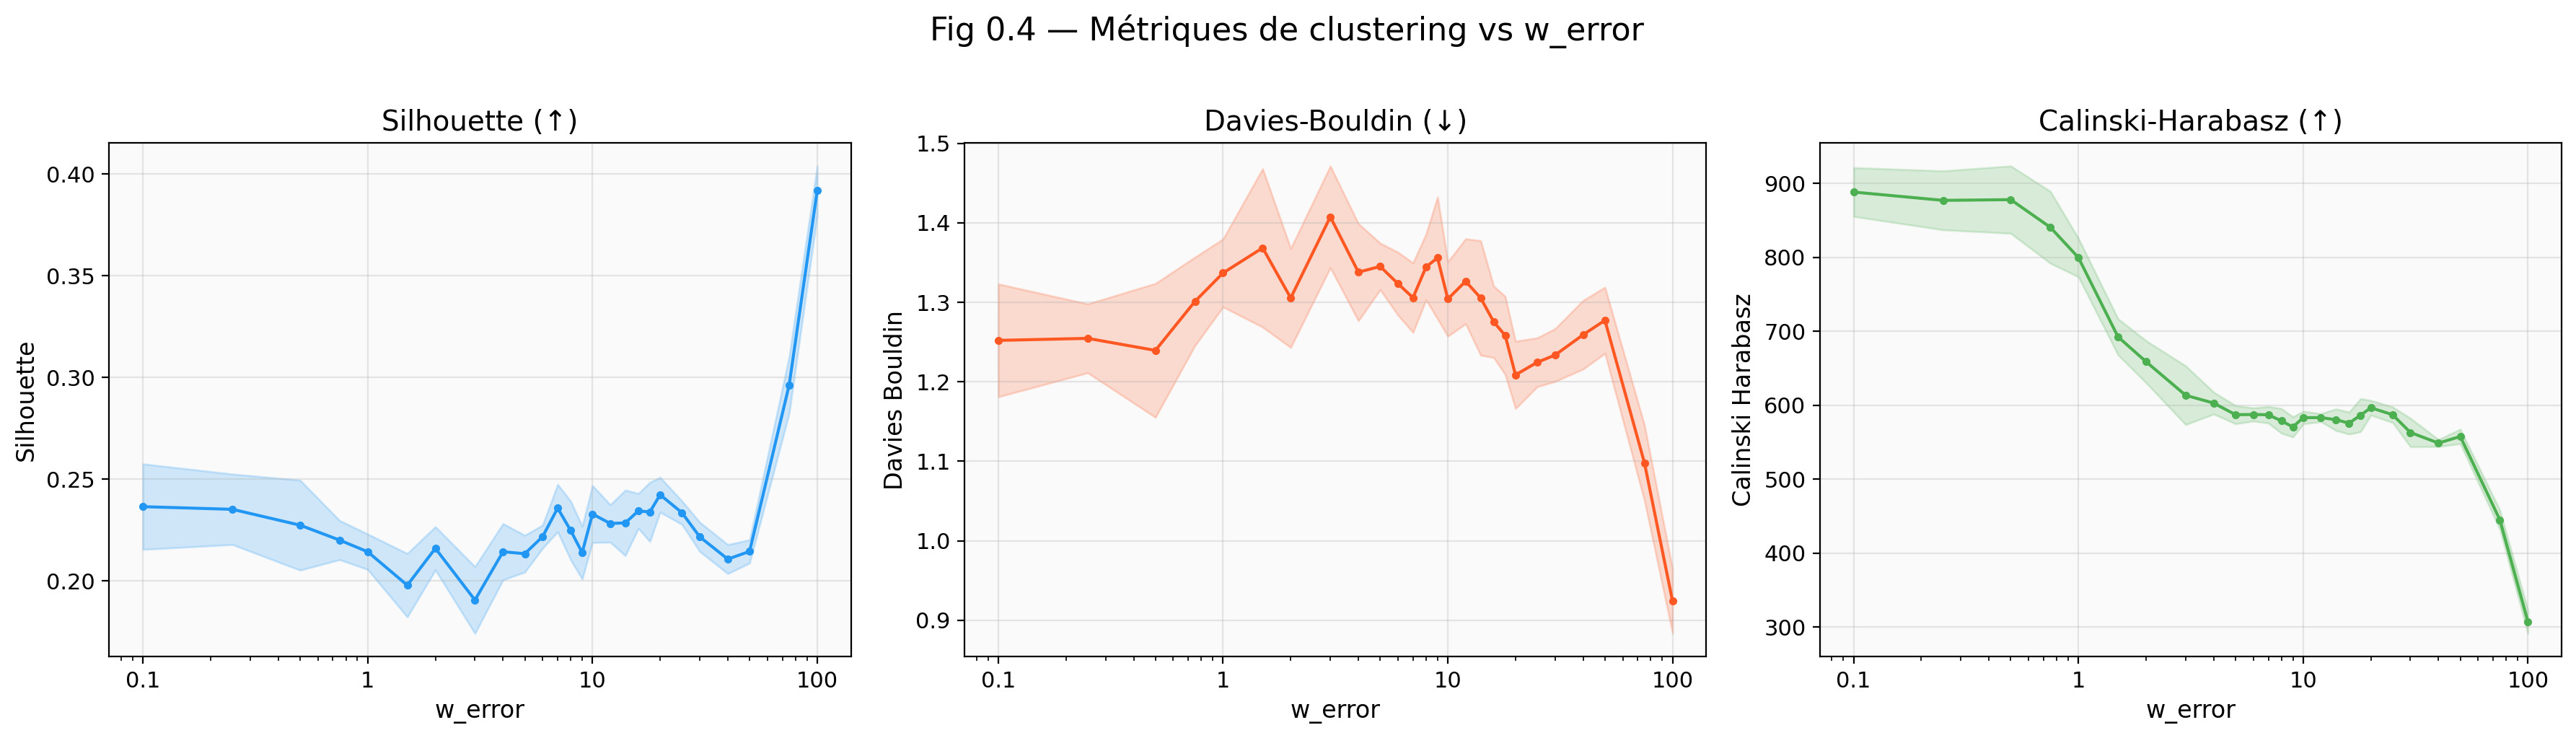
\includegraphics[width=0.9\textwidth, height=0.28\textheight, keepaspectratio]{img/fig0_4_panel_metrics_werror.jpg}
    \caption{Évolution de la qualité topologique du clustering en fonction de $w_{error}$.}
    \label{fig:clustering_werror}
\end{figure}

Pour confirmer ce choix purement spatial, la Figure \ref{fig:clustering_werror} illustre l'impact de la compression sur la qualité future du clustering. L'observation conjointe montre que le score de cohésion (Silhouette \cite{rousseeuw1987}) présente une forte variance pour les petites valeurs de $w_{error}$ avant de se stabiliser autour de $w_{error} \approx 12$. Ce paramètre offre donc un bon compromis entre précision géométrique et qualité du clustering en aval.

\begin{figure}[H]
    \centering
    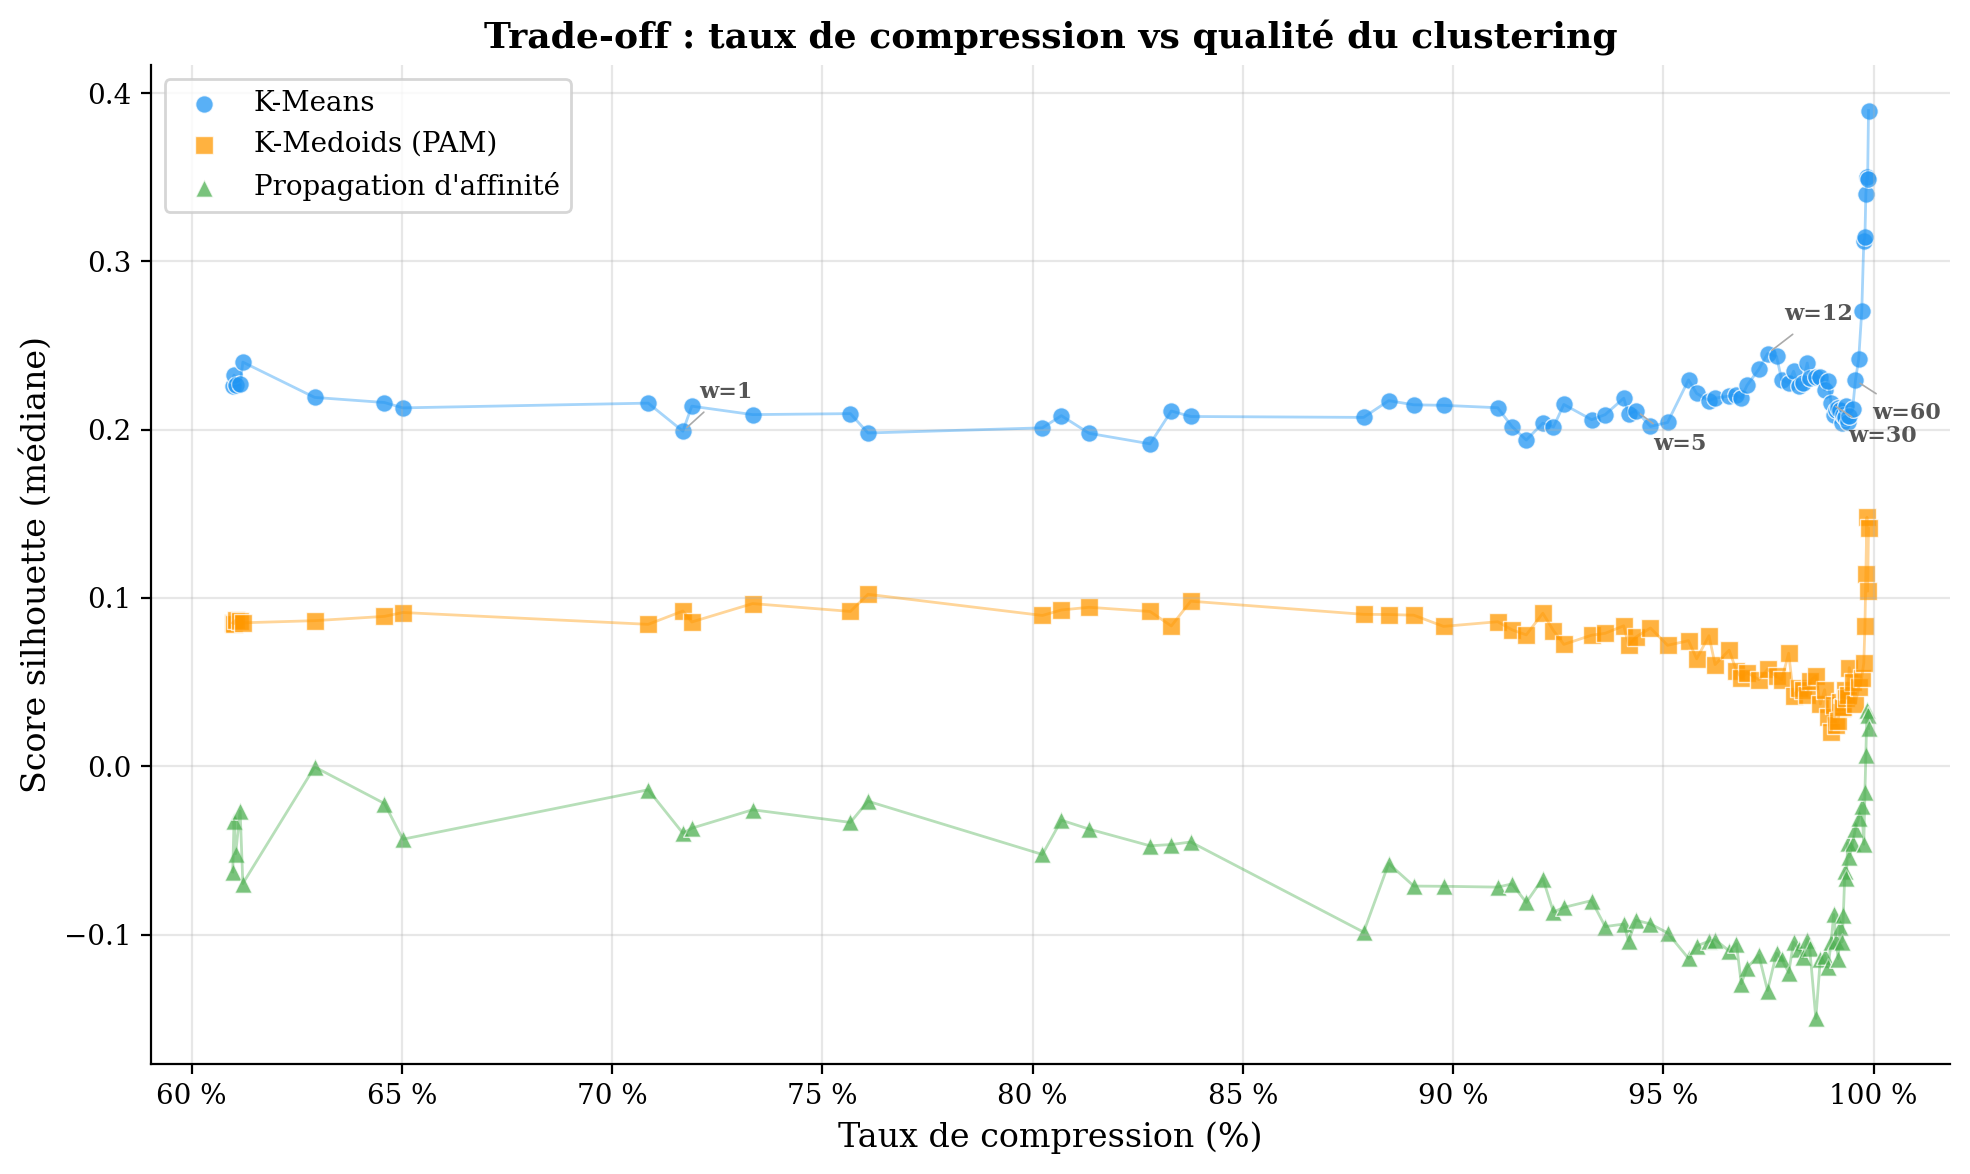
\includegraphics[width=0.85\textwidth]{img/fig13_compression_vs_silhouette.png}
    \caption{Trade-off entre taux de compression et qualité du clustering (score silhouette médian) pour trois algorithmes. Le paramètre $w_{error}=12$ est annoté à $\sim$96\% de compression.}
    \label{fig:compression_vs_silhouette}
\end{figure}

La Figure \ref{fig:compression_vs_silhouette} synthétise ce compromis en traçant directement le score silhouette en fonction du taux de compression pour les trois algorithmes de clustering. On constate que K-Means maintient un score stable ($\sim$0.21) sur toute la plage de compression, tandis que K-Médoïdes et Affinity Propagation sont plus sensibles aux compressions extrêmes ($>$98\%). Au point $w_{error}=12$ ($\sim$96\% de compression), les trois méthodes se situent dans leur zone de stabilité, confirmant que notre choix de paramètre ne dégrade pas la qualité du clustering en aval.

\subsubsection{Robustesse au Bruit Gaussien}

Afin de valider la capacité de l'algorithme MDL à filtrer le bruit intrinsèque aux données de clics, nous avons mené une expérience de robustesse par injection de bruit gaussien $\mathcal{N}(0, \sigma^2)$ avec $\sigma$ croissant de 0 à 20.

\begin{figure}[H]
    \centering
    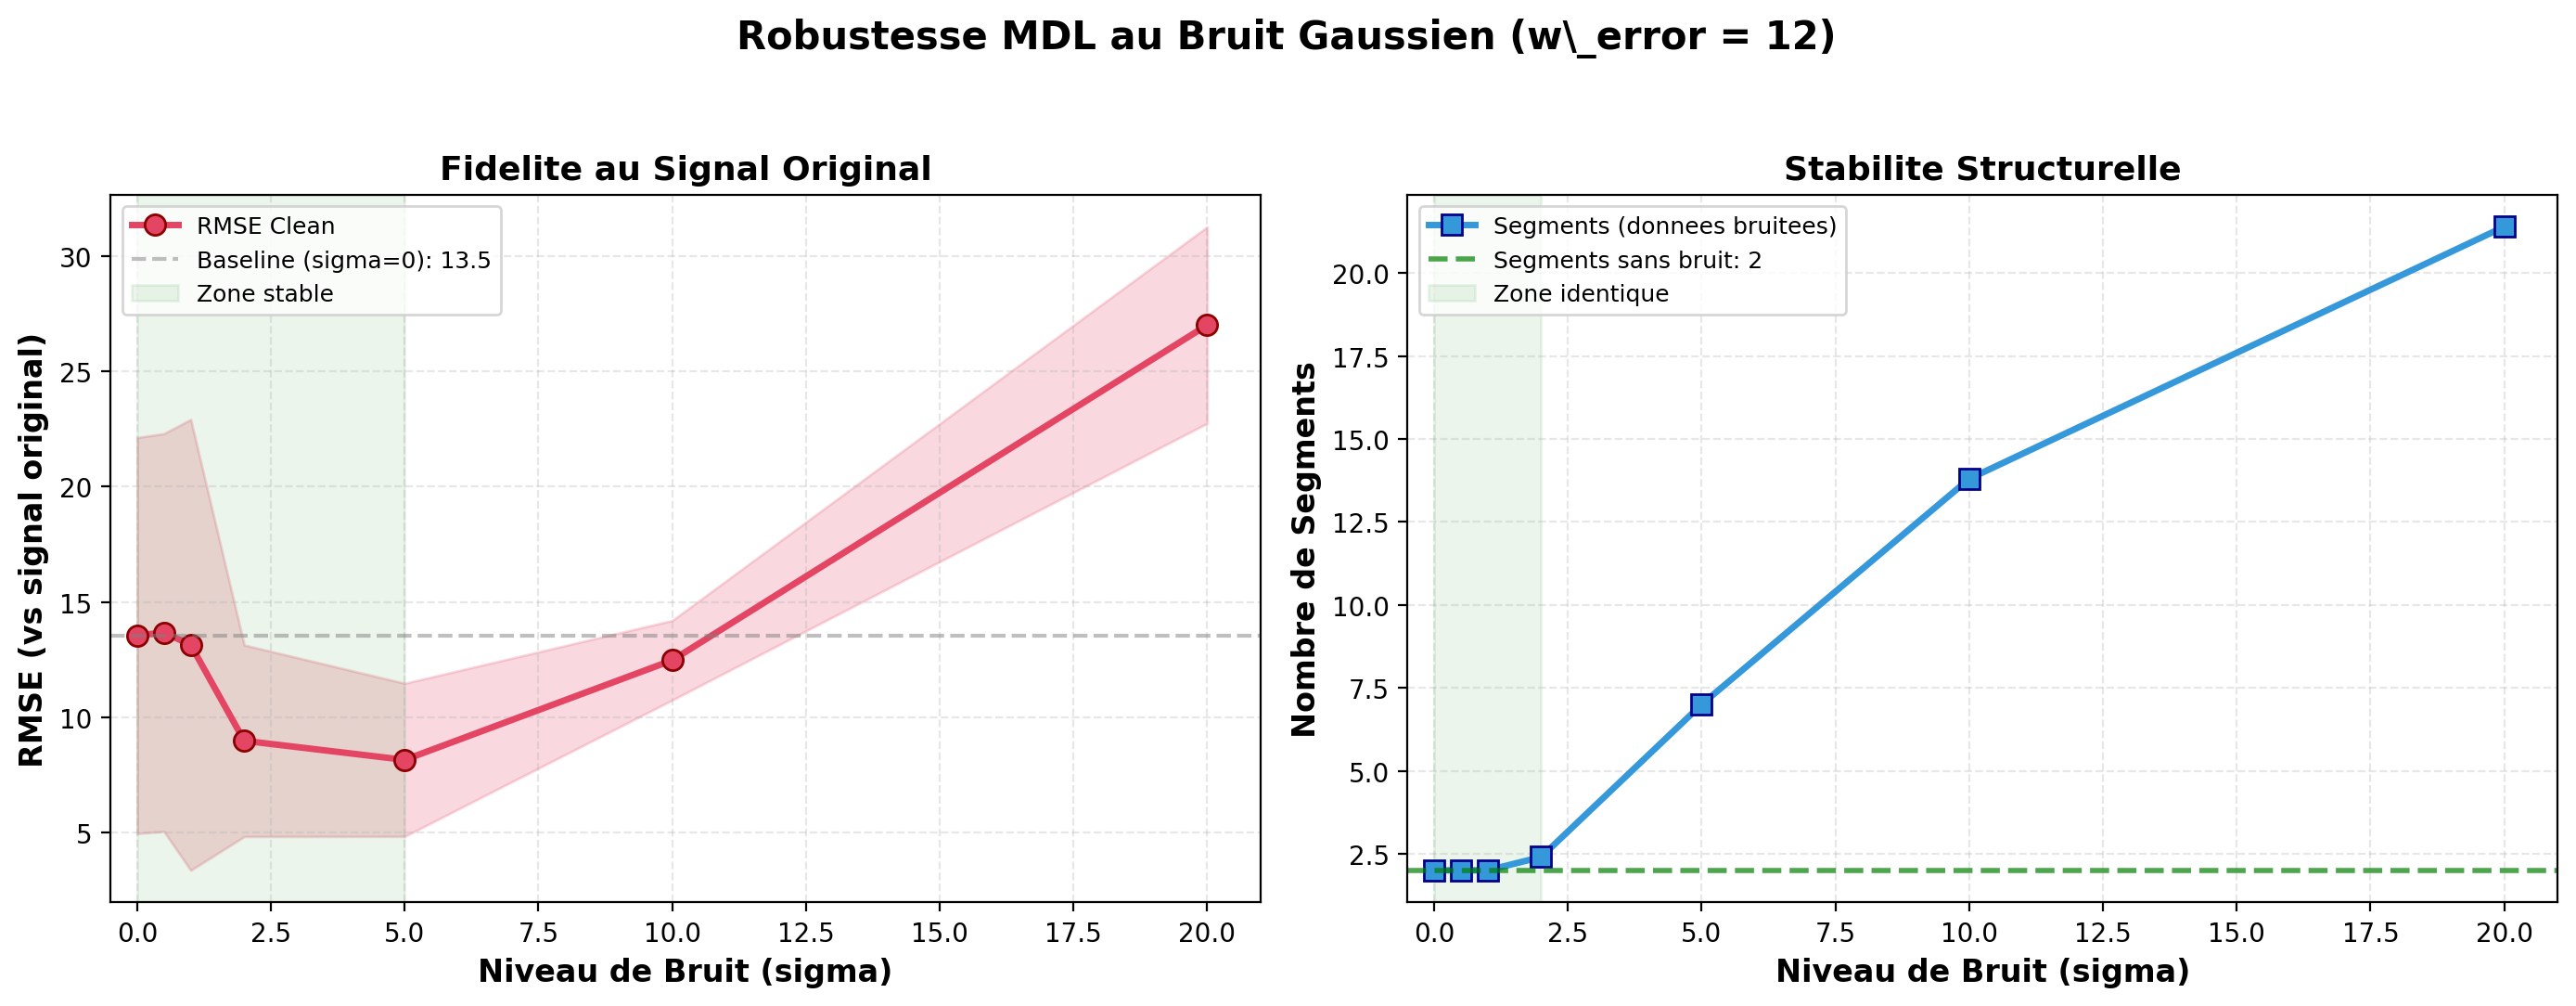
\includegraphics[width=0.9\textwidth, height=0.3\textheight, keepaspectratio]{img/robustesse_bruit_w12.png}
    \caption{Robustesse de la compression MDL ($w_{error}=12$) au bruit gaussien : fidélité au signal original (RMSE Clean) et stabilité structurelle (nombre de segments) en fonction du niveau de bruit $\sigma$.}
    \label{fig:robustesse_bruit}
\end{figure}

Le protocole consiste à extraire 5 échantillons aléatoires (data augmentation), à injecter un bruit gaussien de variance croissante, puis à compresser les données bruitées avec $w_{error}=12$. La RMSE est ensuite mesurée par rapport au signal original (sans bruit).

La Figure \ref{fig:robustesse_bruit} révèle deux résultats importants. Premièrement, le RMSE reste stable — voire diminue légèrement — pour $\sigma \leq 5$, ce qui montre que MDL absorbe les perturbations modérées sans dégrader la fidélité au signal. Deuxièmement, le nombre de segments produits reste identique ($\sim$2 segments) jusqu'à $\sigma = 2$, démontrant une stabilité structurelle remarquable. Ce n'est qu'à partir de $\sigma \geq 10$ que le bruit commence à créer des segments supplémentaires. Ces résultats confirment que l'algorithme MDL agit comme un filtre passe-bas naturel : il élimine le bruit haute fréquence (micro-clics) tout en préservant le signal basse fréquence (déplacements stratégiques).

% ------------------------------------------
% 6.3 : CLUSTERING
% ------------------------------------------
\subsection{Évaluation des Algorithmes de Clustering}

\subsubsection{Optimisation de $k$ : Compromis entre Topologie et Sémantique}

La détermination du nombre de macro-zones ($k$) est une étape critique. Pour éviter un découpage arbitraire, nous avons évalué notre clustering pour $k \in [2, 30]$.

\begin{figure}[H]
    \centering
    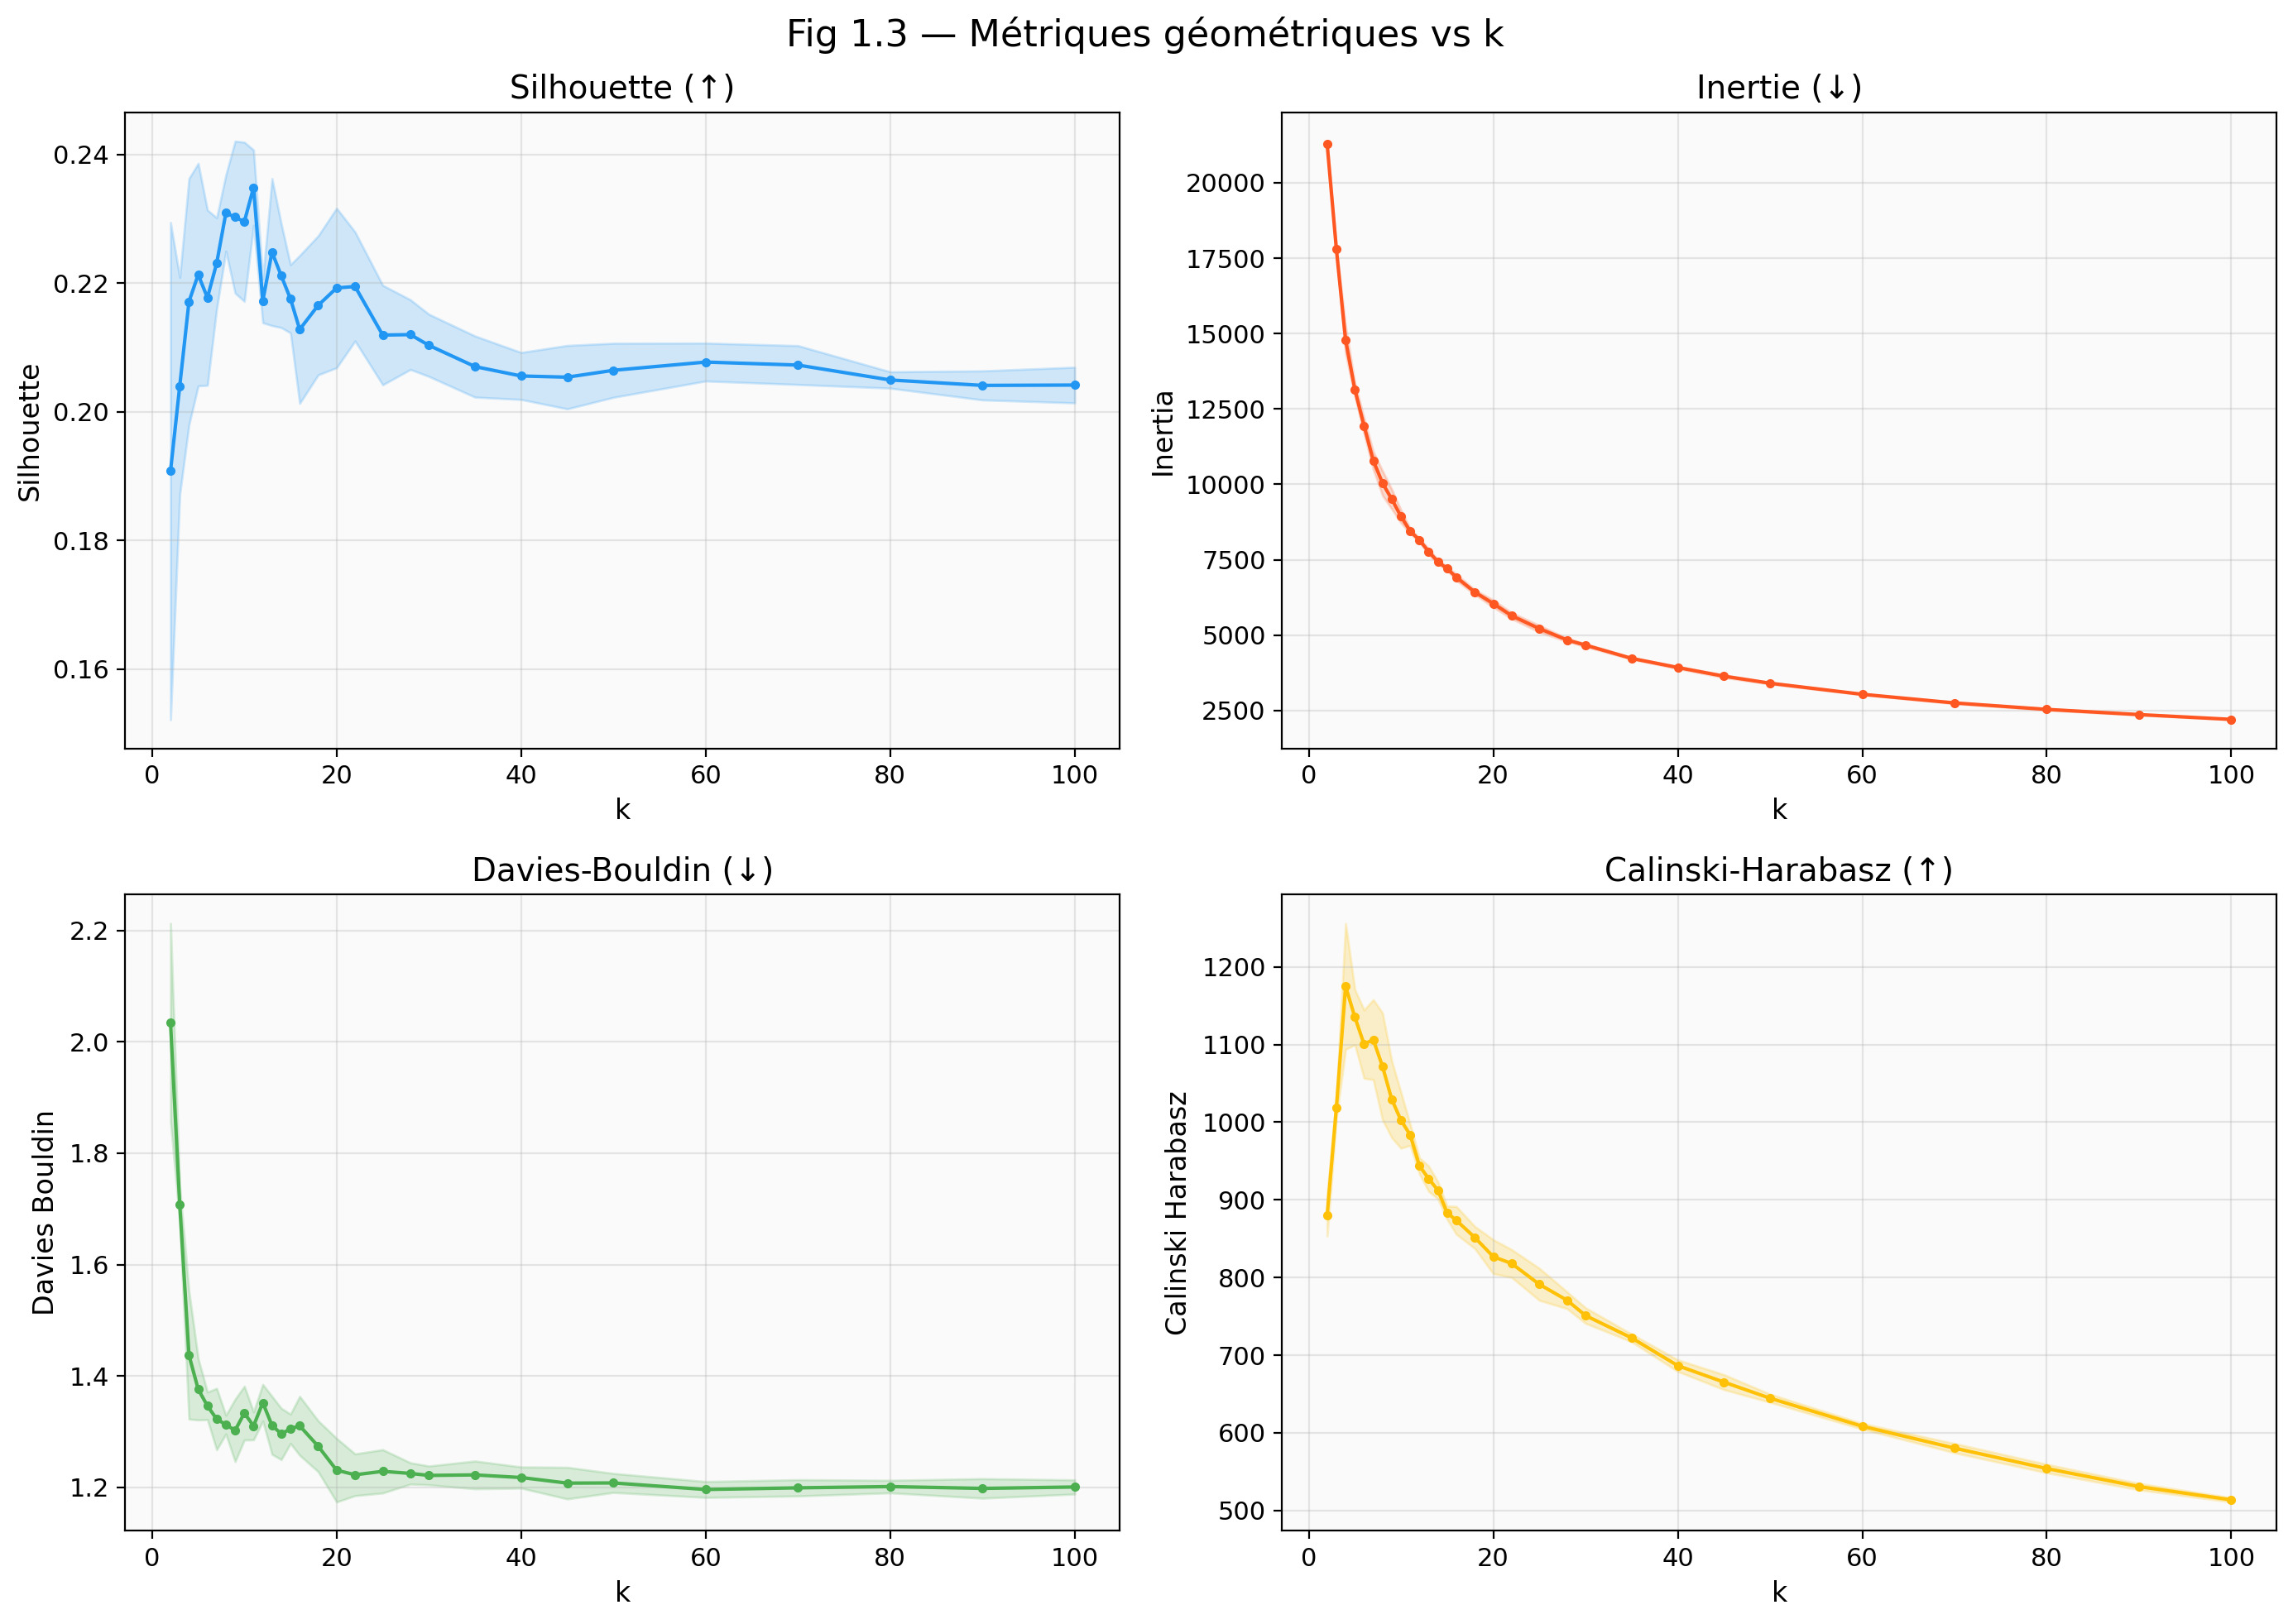
\includegraphics[width=0.9\textwidth, height=0.28\textheight, keepaspectratio]{img/fig1_3_panel_metrics_k.jpg}
    \caption{Évaluation multi-métriques géométriques pour la recherche du $k$ optimal.}
    \label{fig:geometric_k}
\end{figure}

La Figure \ref{fig:geometric_k} illustre les métriques géométriques classiques. On observe une "cassure" typique (méthode du coude) : le score d'erreur de Davies-Bouldin atteint un point bas et le score de Silhouette maintient un plateau acceptable autour de $k=10$. 

\begin{figure}[H]
    \centering
    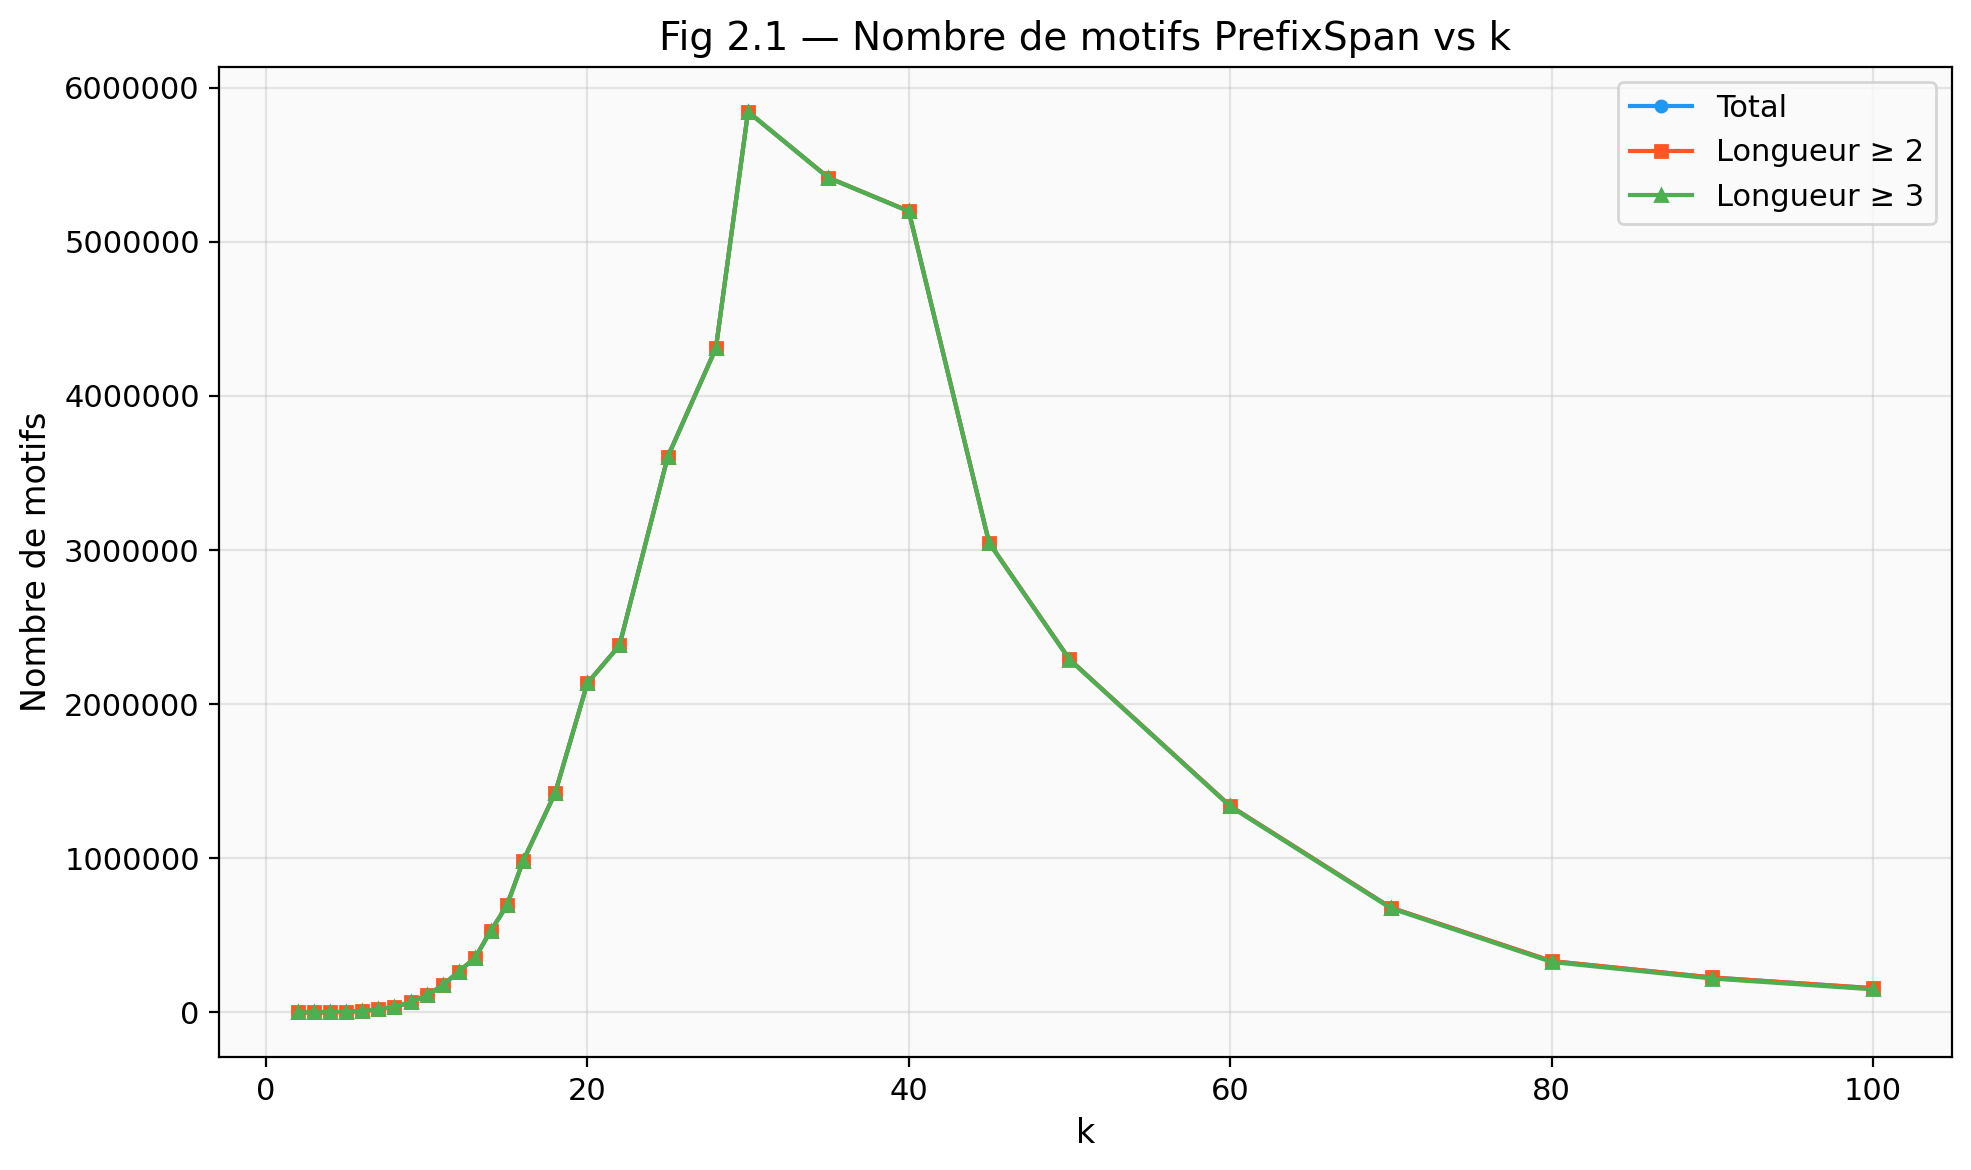
\includegraphics[width=0.8\textwidth, height=0.28\textheight, keepaspectratio]{img/fig2_1_nb_motifs_k.jpg}
    \caption{Évolution du nombre de motifs séquentiels extraits en fonction de $k$.}
    \label{fig:semantic_motifs}
\end{figure}

Pour vérifier que cette topologie a un sens stratégique, la Figure \ref{fig:semantic_motifs} mesure l'impact de $k$ sur le volume de stratégies extraites par PrefixSpan. On remarque qu'à $k=10$, l'algorithme génère un volume riche mais maîtrisé de motifs pertinents, évitant l'explosion combinatoire générée par une sur-segmentation. Le paramètre $k=10$ apparaît donc comme le meilleur compromis empirique entre richesse et lisibilité des résultats.

\subsubsection{Évaluation Topologique Comparative des Algorithmes}

Afin de sélectionner le modèle final, nous avons mis en compétition nos trois algorithmes spatiaux. 

\begin{figure}[H]
    \centering
    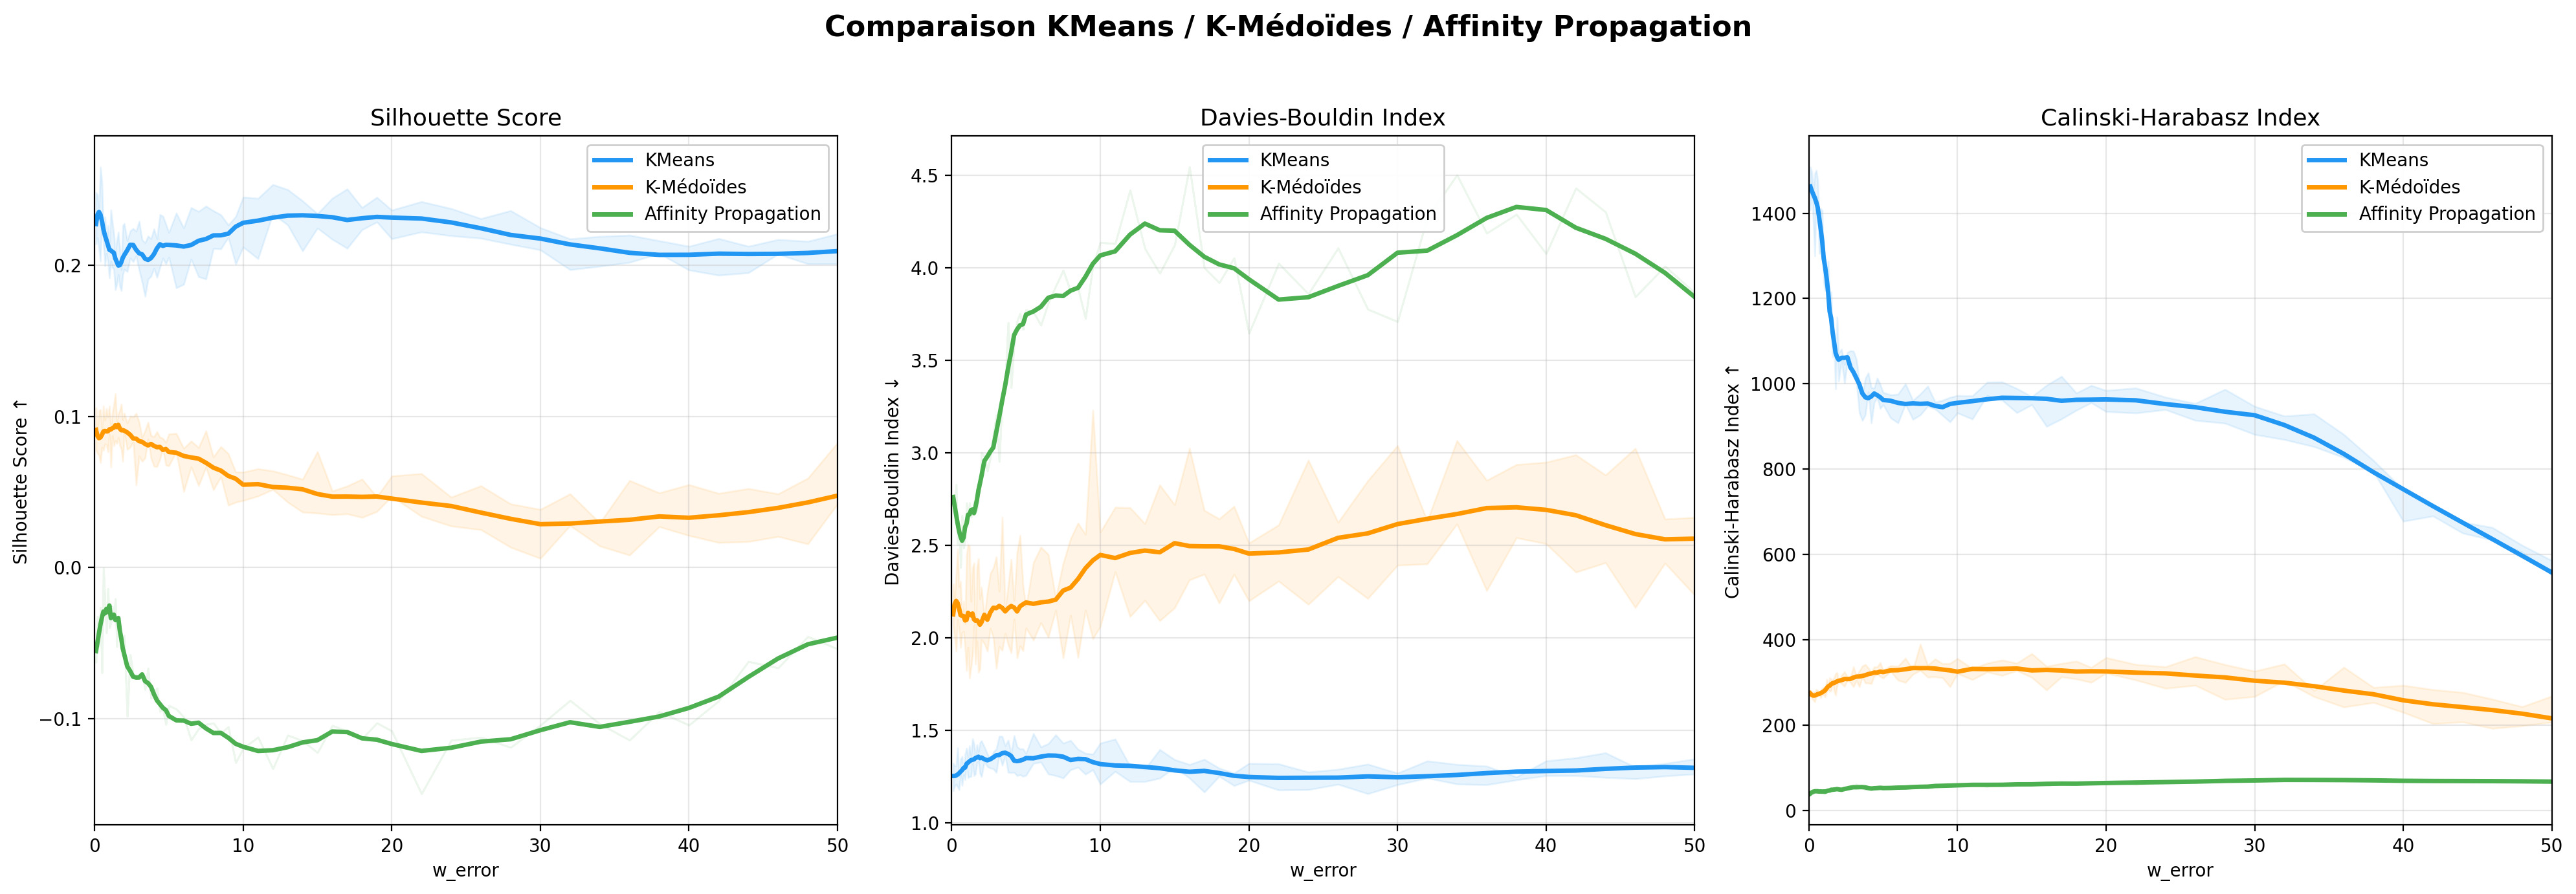
\includegraphics[width=0.9\textwidth, height=0.3\textheight, keepaspectratio]{img/fig3_comparison_algo.jpg}
    \caption{Comparaison globale (Silhouette, Davies-Bouldin, Calinski-Harabasz) des 3 algorithmes.}
    \label{fig:clustering_quality}
\end{figure}

Le graphique en barres (Figure \ref{fig:clustering_quality}) montre de meilleures performances relatives de K-Médoïdes et de l'Affinity Propagation par rapport à K-Means. Par exemple, K-Médoïdes affiche un score de Silhouette de $\sim 0.14$ contre $0.08$ pour K-Means. Il faut noter que ces valeurs restent globalement basses (un score de Silhouette supérieur à $0.5$ indiquerait une structure de clusters bien séparée), ce qui s'explique par la nature dense et chevauchante des trajectoires spatiales. Néanmoins, la différence relative s'explique : K-Means ne peut moyenner que des coordonnées brutes euclidiennes, tandis que nos deux algorithmes avancés exploitent directement la matrice de distance experte (TRACLUS), respectant ainsi la perpendicularité et le sens des trajectoires.

\subsubsection{Analyse de Sensibilité et Robustesse de la Propagation d'Affinité (AP)}
La topologie finale de la Propagation d'Affinité dépend fortement du paramètre de \textit{preference} et de la volumétrie des données ($N$).

\begin{figure}[H]
    \centering
    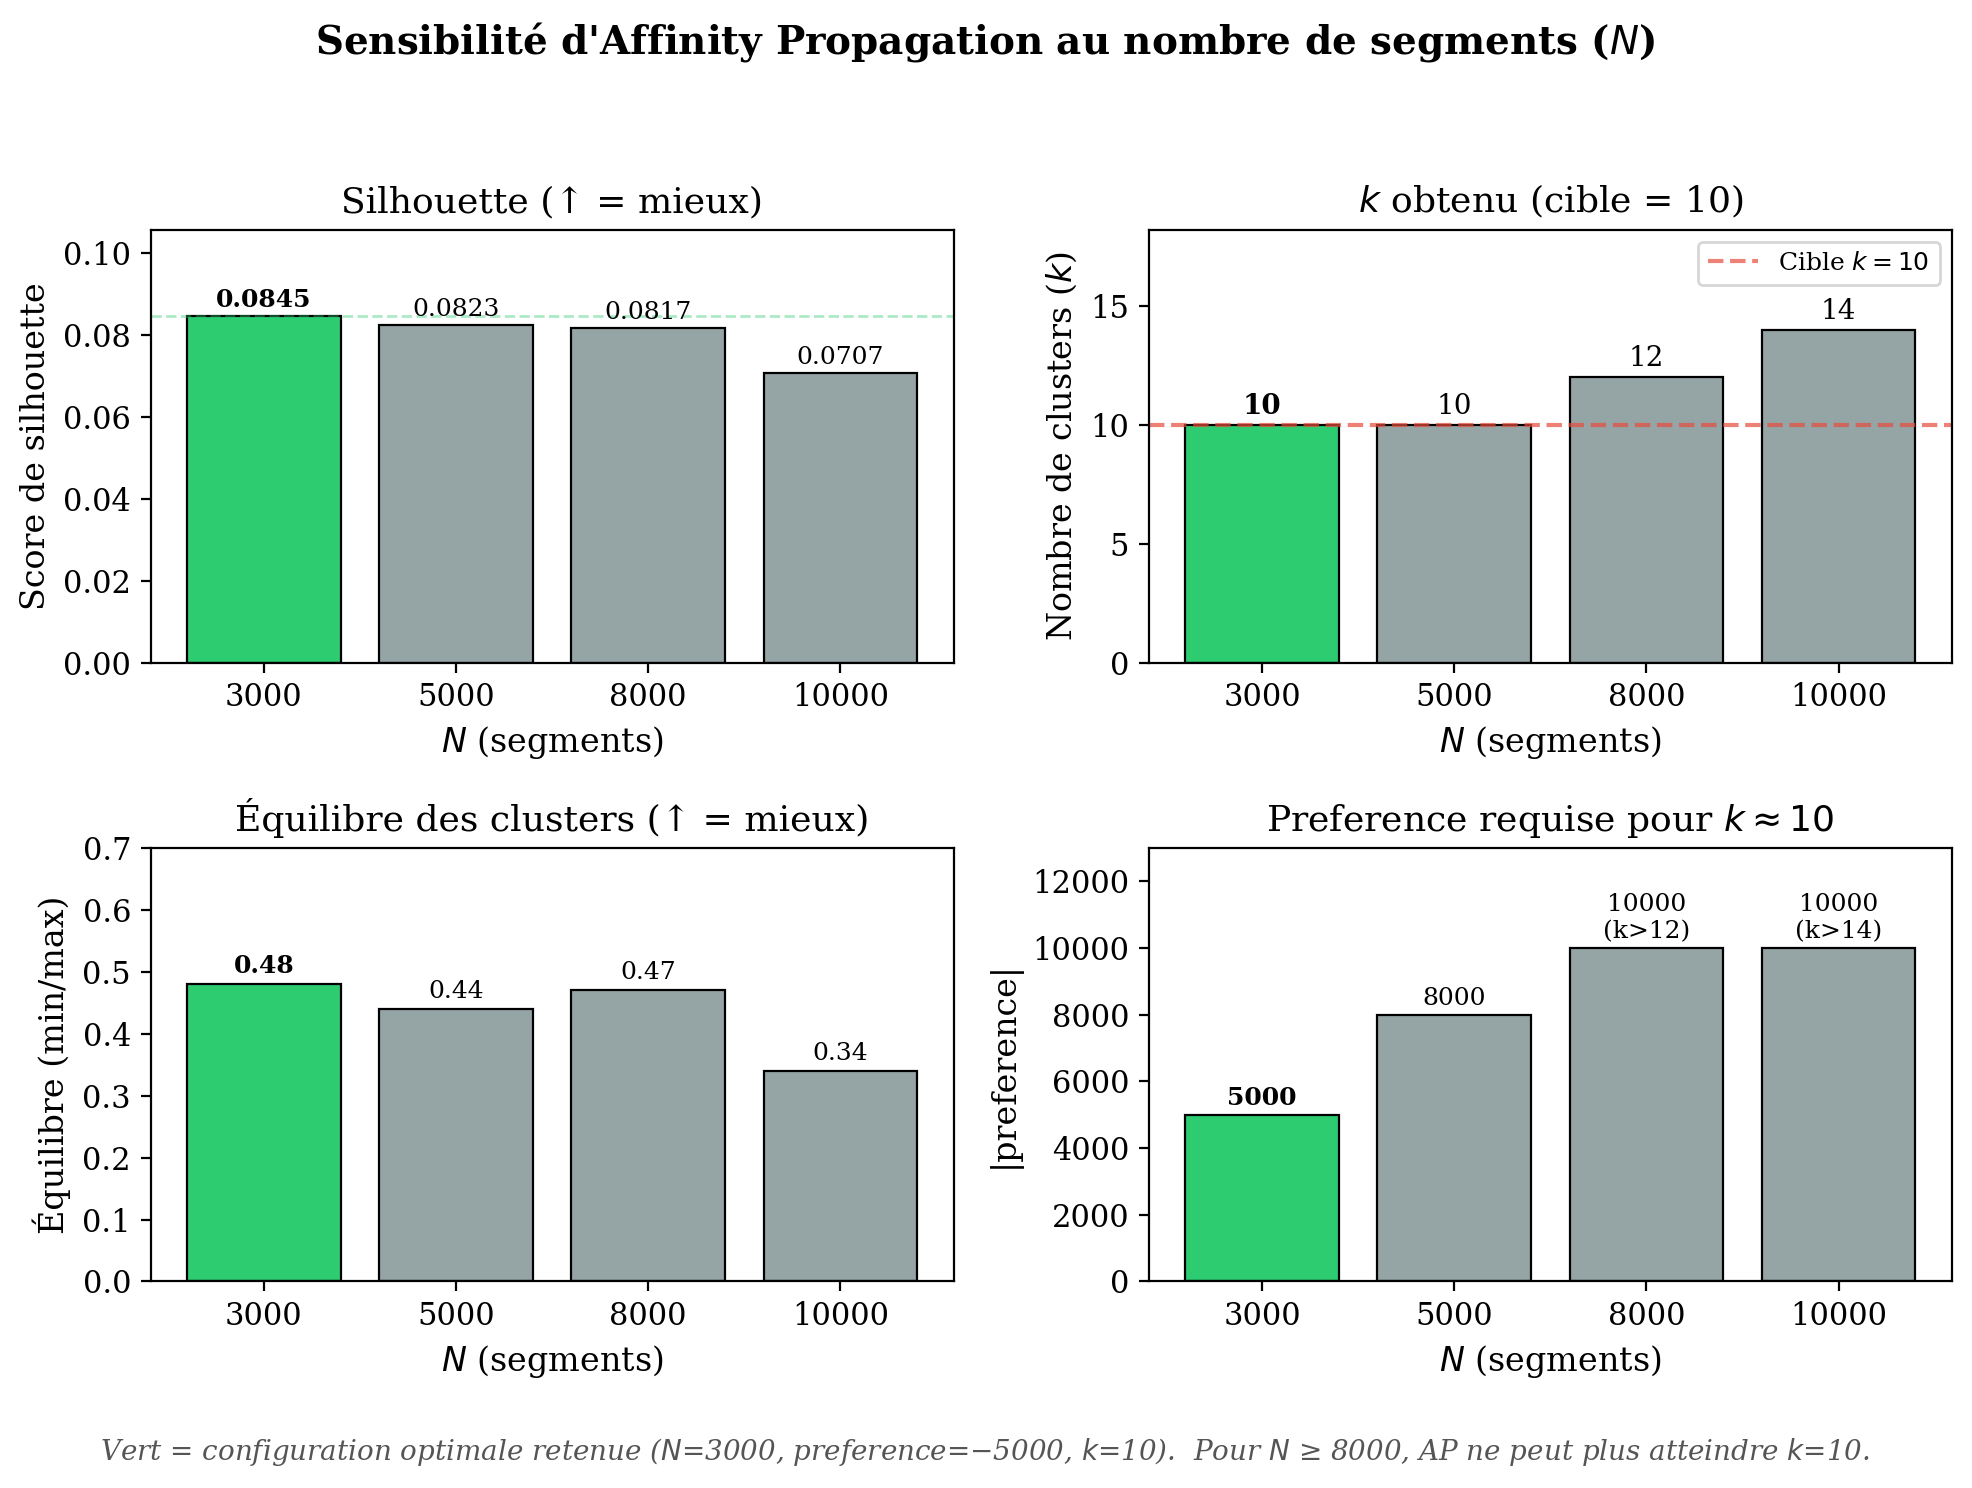
\includegraphics[width=\textwidth, height=0.3\textheight, keepaspectratio]{img/ap_N.jpg}
    \caption{Étude de sensibilité de l'Affinity Propagation au volume de données ($N$) et à la préférence.}
    \label{fig:ap_sensitivity}
\end{figure}

L'analyse de la Figure \ref{fig:ap_sensitivity} révèle une dégradation structurelle lors du passage à l'échelle :
\begin{itemize}
    \item \textbf{La rupture de topologie ($k$ obtenu) :} Pour un échantillon de $N=3000$ segments, l'AP converge parfaitement vers notre cible de 10 clusters. Au-delà de $N \ge 8000$, l'algorithme subit une sur-segmentation forcée (12 à 14 clusters), refusant de fusionner ces micro-déplacements même sous une contrainte de \textit{preference} extrême ($-10 000$).
    \item \textbf{La chute de cohésion spatiale :} L'augmentation du volume de données fait chuter de manière linéaire la qualité géométrique (baisse de Silhouette) et l'équilibre massique des clusters.
\end{itemize}

Ce test montre que le sous-échantillonnage à $N=3000$ segments constitue un bon compromis permettant à l'AP de produire un découpage cohérent de la carte de \textit{DotA 2} sans être perturbé par le bruit.

\subsubsection{Scalabilité vs Qualité Sémantique : Le Choix Final}

K-Médoïdes s'exécute extrêmement rapidement ($\sim 0.03s$). À l'inverse, l'Affinity Propagation (AP) voit son temps de convergence propre exploser ($\sim 6s$ sur 3000 segments) en raison de sa complexité quadratique $\mathcal{O}(N^2)$. 

Cependant, une inspection géographique révèle une faille structurelle majeure de K-Médoïdes sur nos données :
\begin{itemize}
    \item \textbf{L'anomalie du doublon K-Médoïdes :} L'algorithme place deux centres de clusters à seulement 5 unités d'écart, gaspillant un cluster pour désigner la même zone (l'Offlane Radiant) tout en ignorant la Top Lane.
    \item \textbf{La supériorité géographique de l'AP :} L'AP identifie 10 zones géographiques distinctes, sans doublon constaté.
\end{itemize}

\textbf{Bilan :} Si K-Médoïdes est le seul algorithme viable pour le \textit{Big Data}, l'Affinity Propagation produit le découpage spatial le plus cohérent géographiquement. Notre étape PrefixSpan opérant sur un échantillon de 30 matchs, \textbf{nous utiliserons les clusters générés par l'Affinity Propagation} pour garantir l'extraction de stratégies sémantiquement valides.

% ------------------------------------------
% 6.4 : PREFIXSPAN
% ------------------------------------------
\subsection{Fouille de Motifs Séquentiels et Interprétation Stratégique}

\subsubsection{Gestion de la Volumétrie et Malédiction des Séquences Longues}
Sur des matchs complets, les séquences atteignent environ 65 transitions par joueur. PrefixSpan génère alors un très grand nombre de motifs (près de 100 000, dont la majorité triviaux avec un support $> 95\%$). Pour extraire des motifs plus discriminants, nous avons appliqué un seuil de support minimum de $15\%$ et réalisé la fouille sur un échantillon de 30 matchs. Une compression des états contigus (Run-Length Encoding) a été appliquée pour supprimer le bruit de stationnement.

\subsubsection{Analyse des Motifs Séquentiels (PrefixSpan) et Graphe de Markov}

Avant d'extraire les motifs séquentiels complets, nous avons généré un Graphe de Markov (Figure \ref{fig:markov_graph}). Ce réseau offre une excellente cartographie visuelle des probabilités de transition immédiates (paires) entre nos différentes zones. Cependant, la chaîne de Markov est "sans mémoire" et ne voit pas les séquences longues. La véritable puissance de PrefixSpan réside précisément dans sa capacité à identifier des sous-séquences profondes (longueur $\ge 3$) extraites des trajectoires.

\begin{figure}[H]
    \centering
    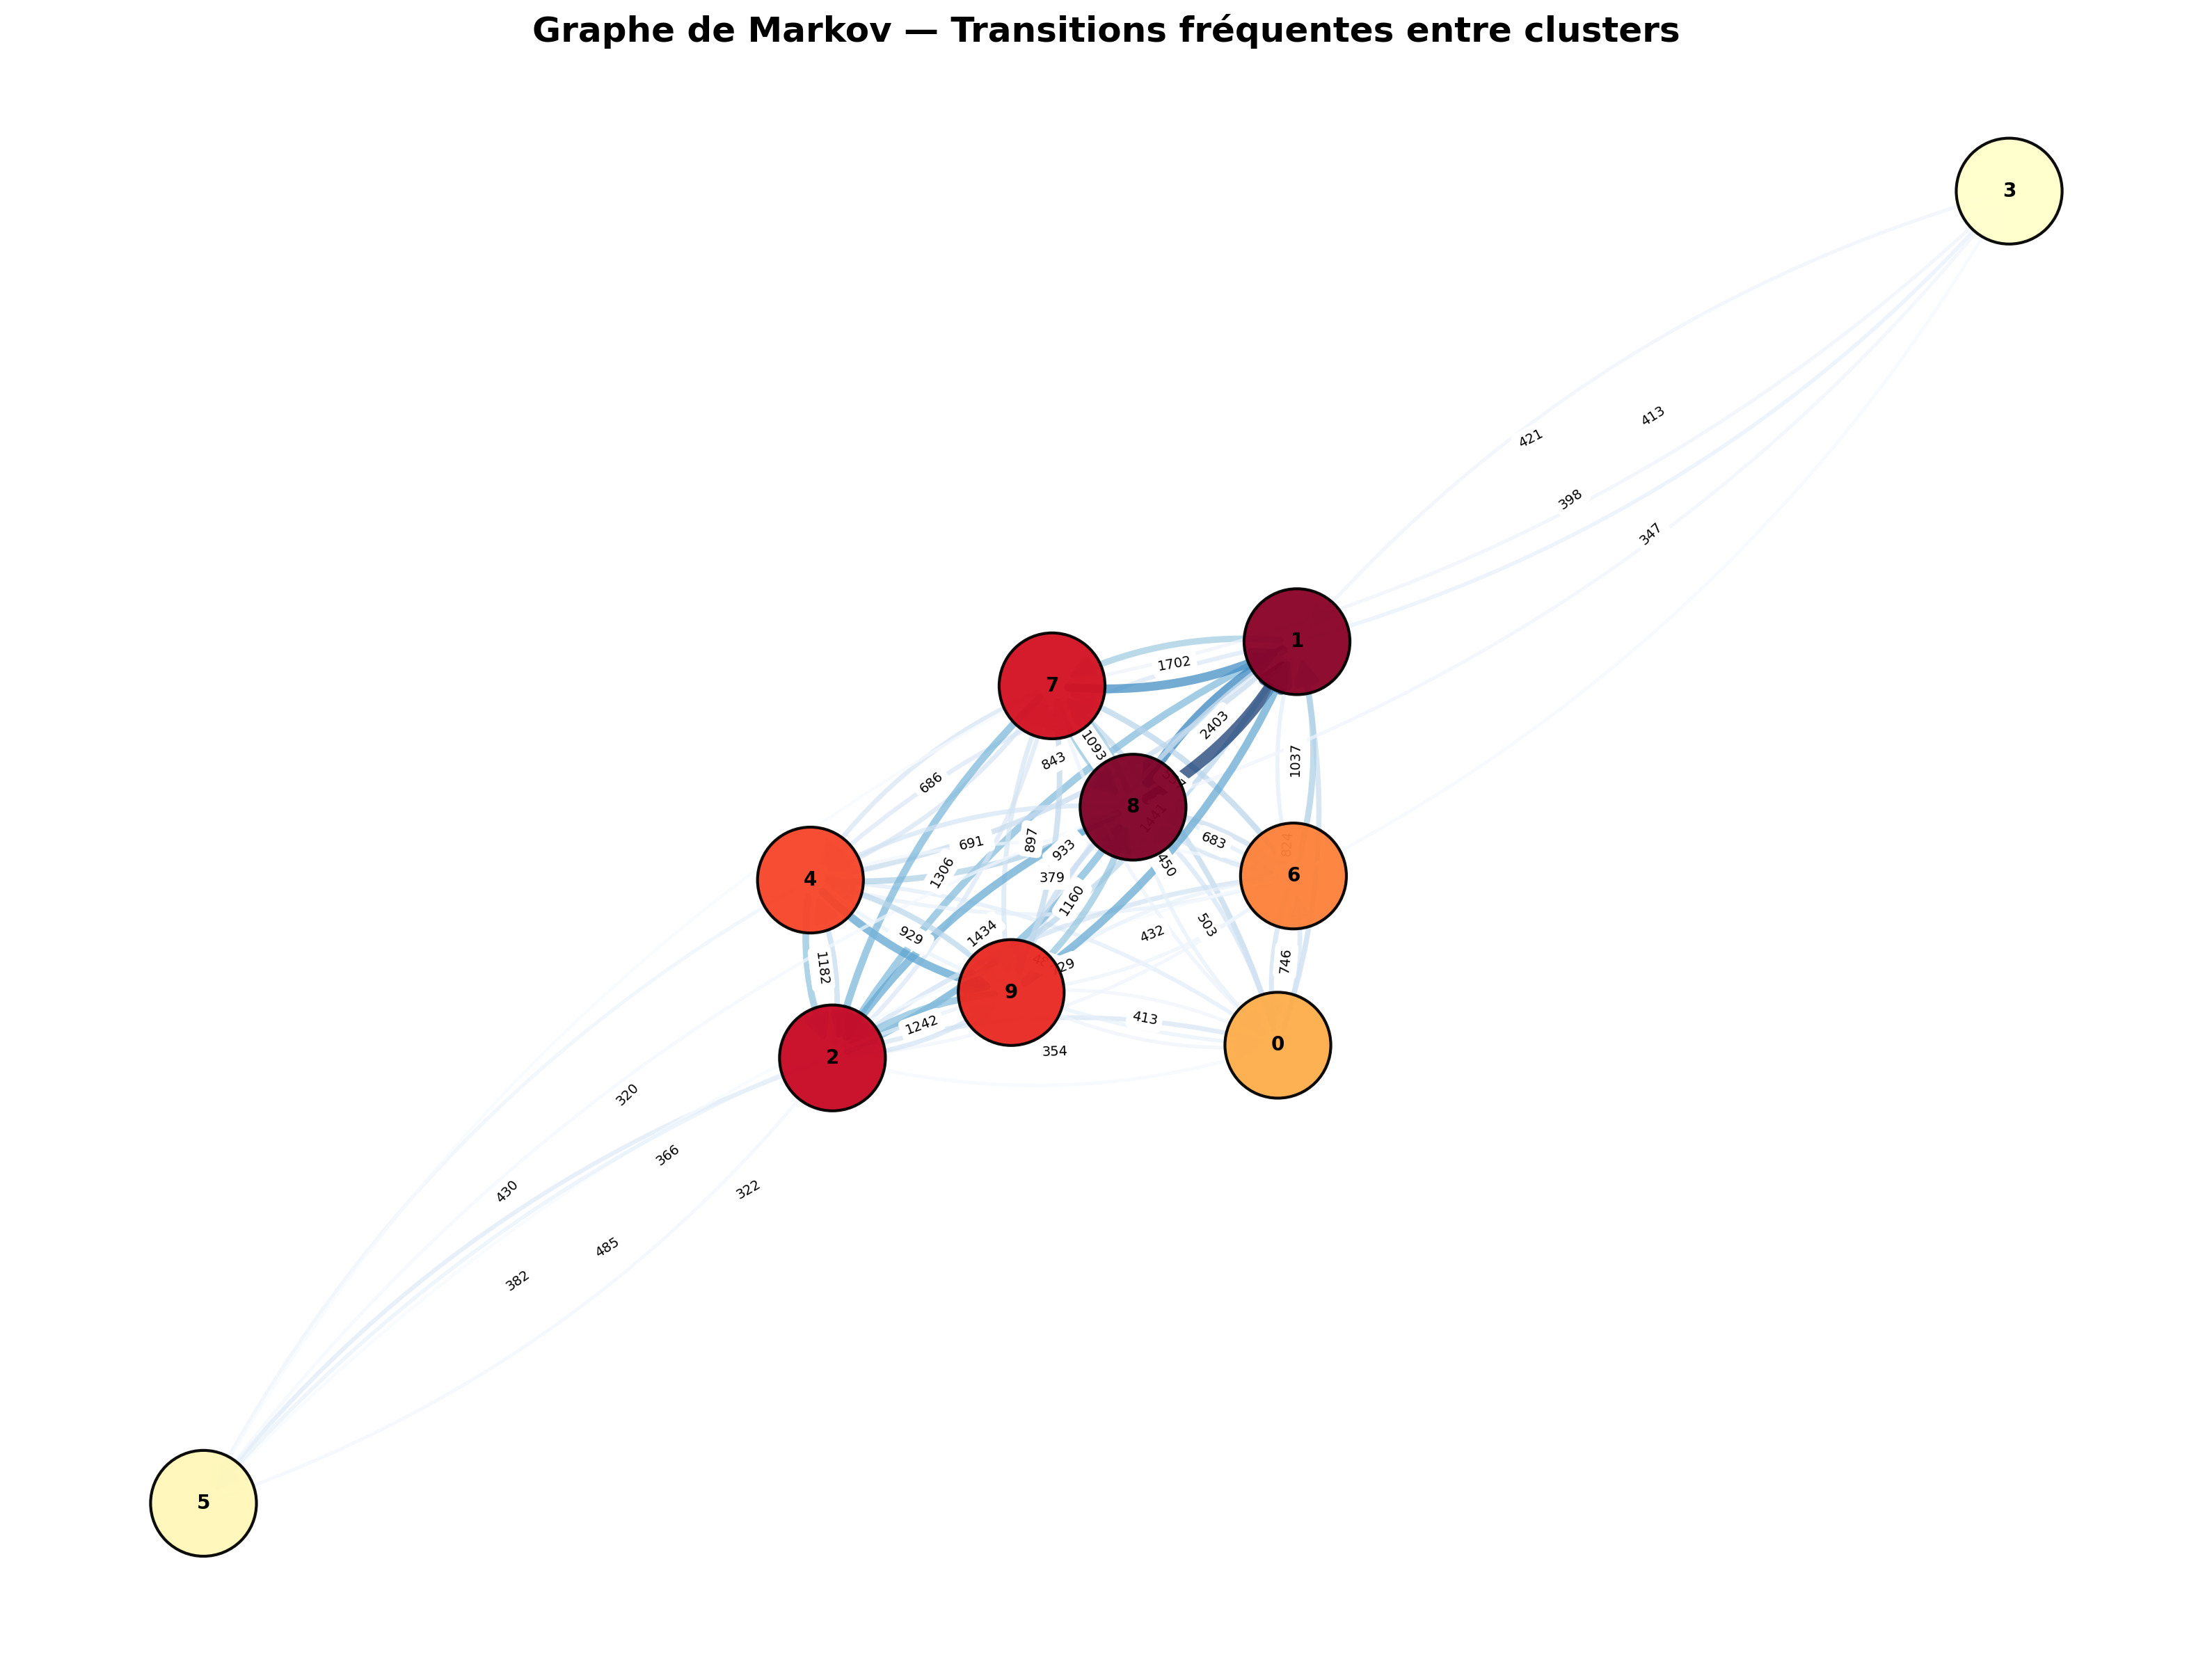
\includegraphics[width=0.85\textwidth, height=0.28\textheight, keepaspectratio]{img/fig3_2_markov_graph.jpg}
    \caption{Graphe de Markov illustrant les probabilités de transition immédiates (paires) entre clusters AP.}
    \label{fig:markov_graph}
\end{figure}

Afin d'éviter la sur-interprétation des motifs (ex: $8 \rightarrow 1$), nous avons systématiquement confronté ces séquences mathématiques à la réalité géographique du terrain, en projetant les centres de nos 10 clusters sur la carte officielle du jeu (Figure \ref{fig:fig3_1_clusters}). 

\begin{figure}[H]
    \centering
    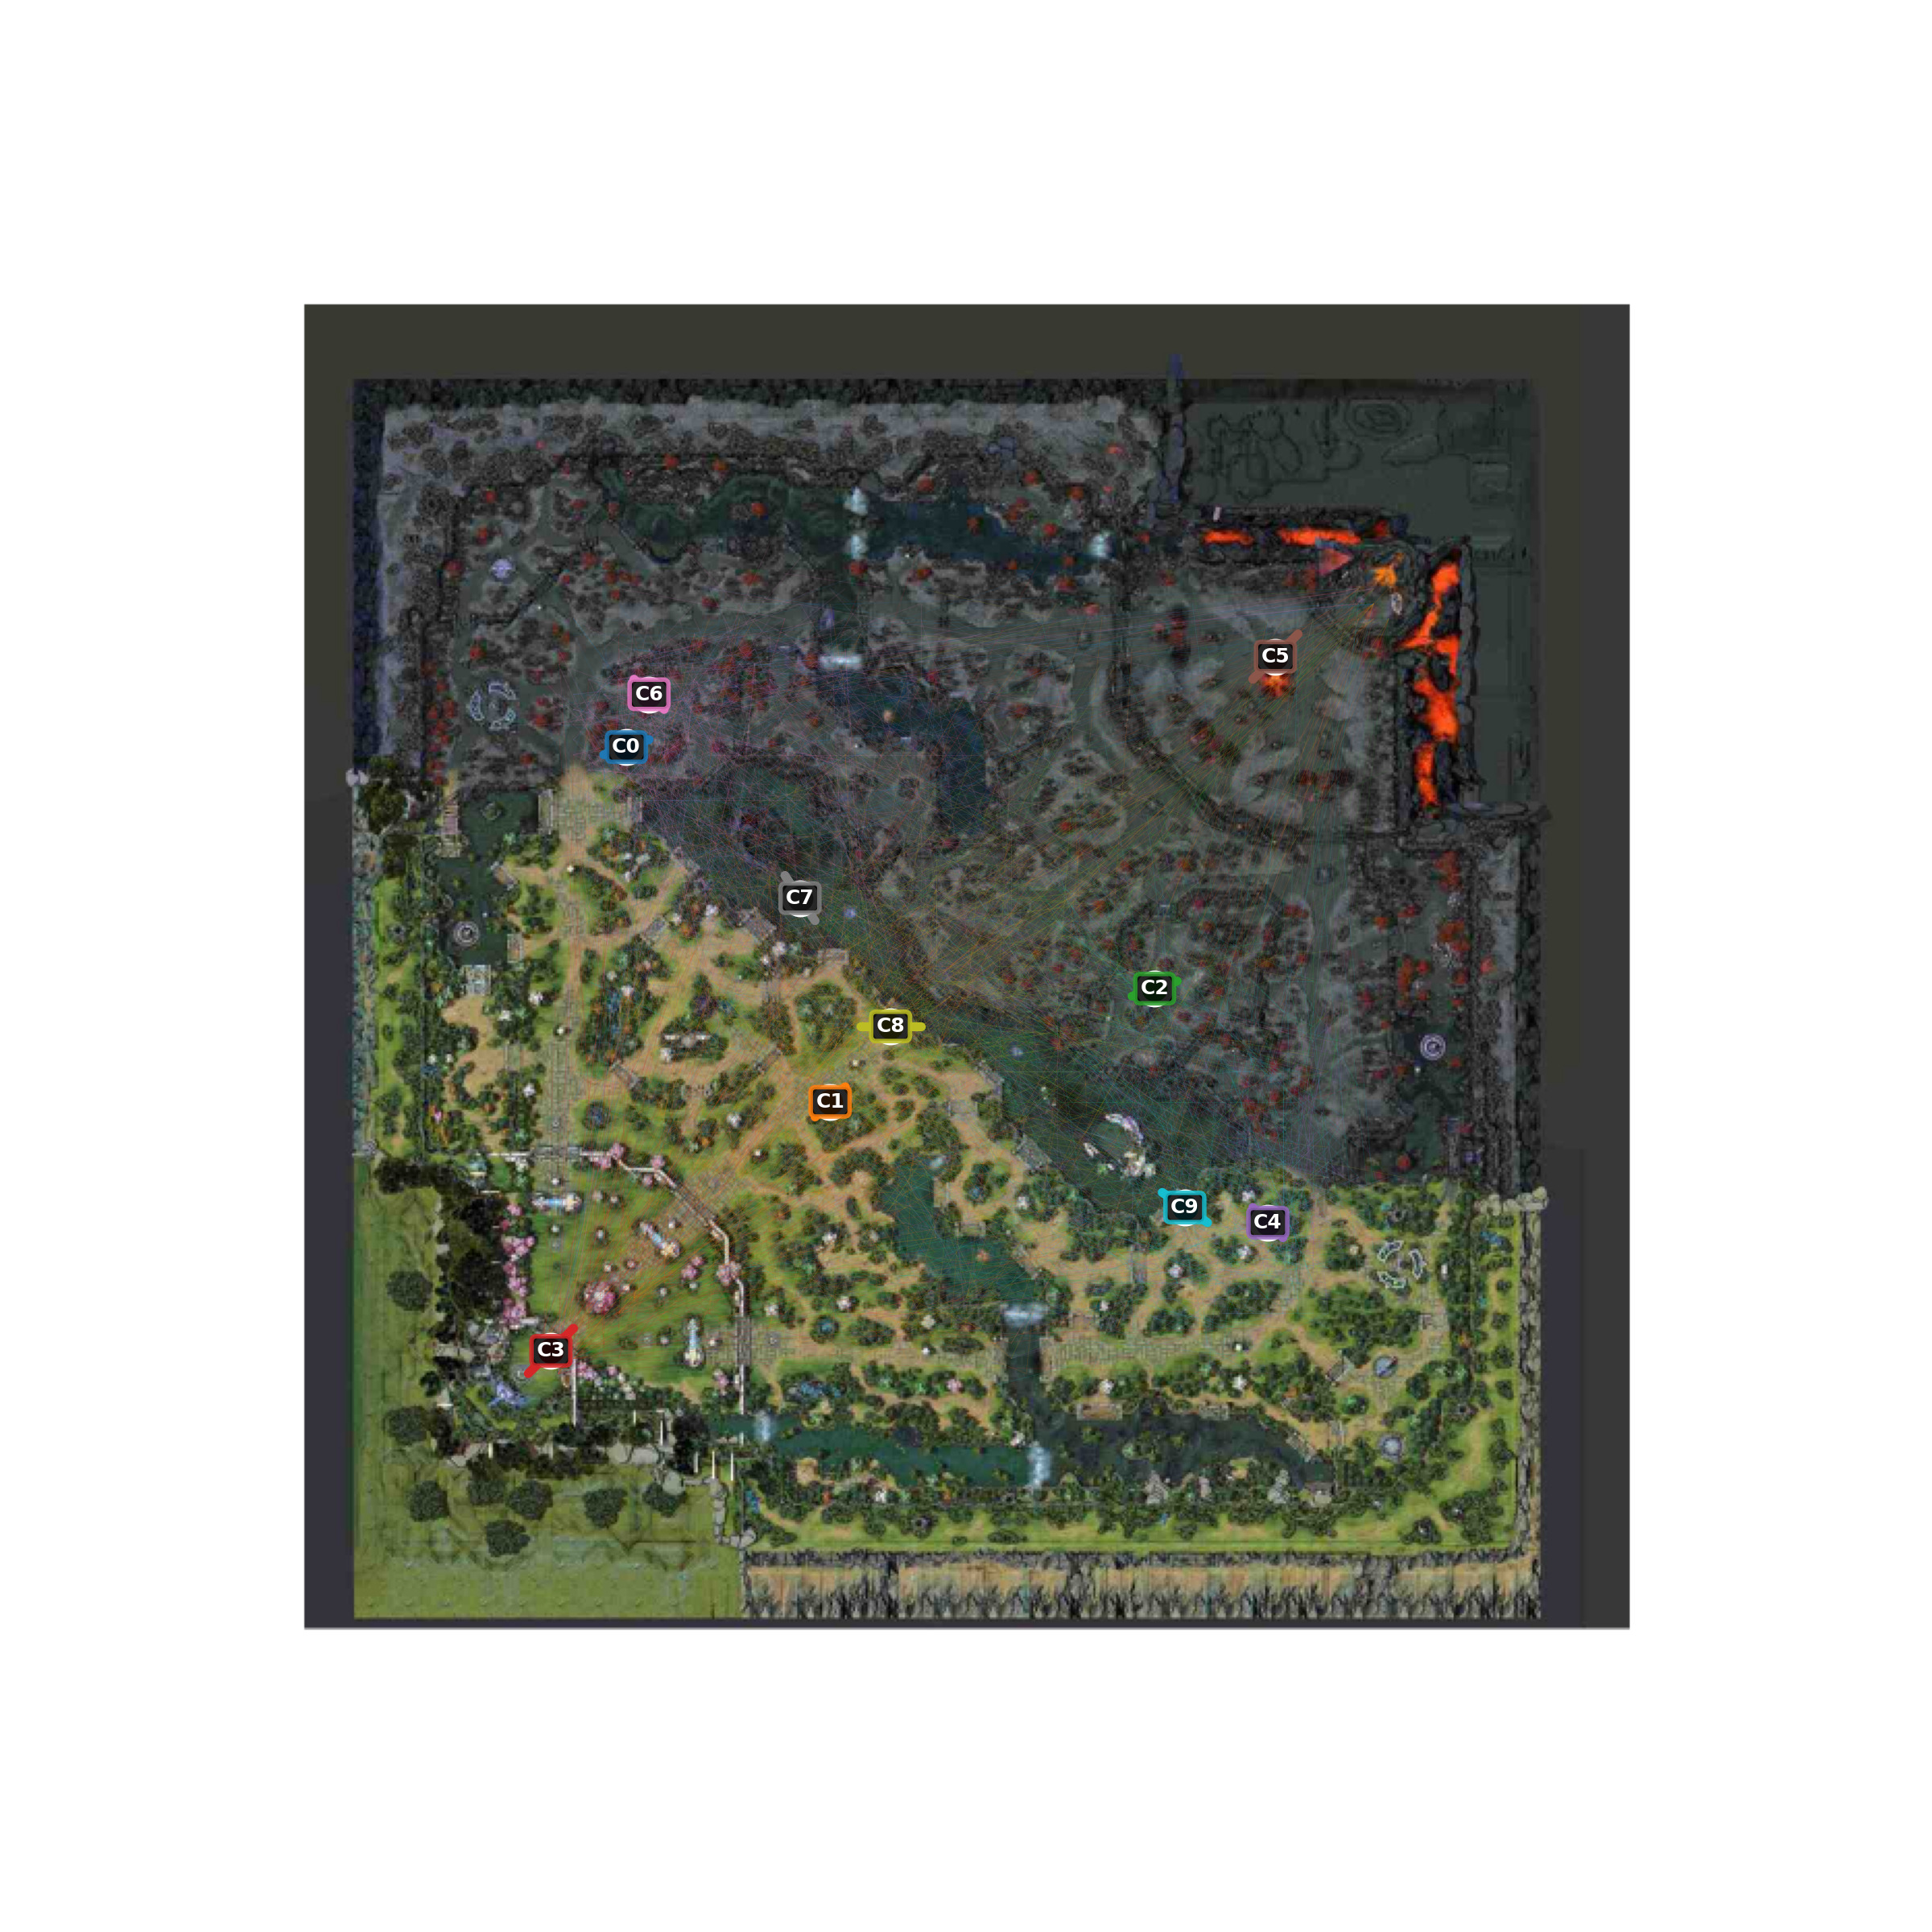
\includegraphics[width=0.8\textwidth, height=0.28\textheight, keepaspectratio]{img/fig3_1_clusters_map.jpg}
    \caption{Cartographie des clusters extraits par Affinity Propagation sur la carte de DotA 2.}
    \label{fig:fig3_1_clusters}
\end{figure}

L'analyse de l'algorithme PrefixSpan, combinée à cette carte, met en lumière les dynamiques séquentielles suivantes :

\begin{itemize}
    \item \textbf{La convergence vers la Rivière et la Safelane (Motifs de longueur $\ge 2$)~:}
    Les 5 motifs de longueur 2 les plus fréquents (support $> 33\%$) se terminent de façon récurrente par les clusters 1 (Rivière) ou 2 (Safelane Dire). Par exemple, les motifs $8 \rightarrow 1$ ($38.6\%$) ou $8 \rightarrow 2$ ($36.9\%$). Le cluster 8 (Midlane) agit ici comme un point de départ majeur et non d'arrivée. Cela est cohérent empiriquement avec la dynamique de \textit{DotA 2} : la Rivière et les lignes principales sont des puits de gravité stratégiques de la carte, carrefours inévitables pour la prise d'objectifs (Runes, Roshan).

    \item \textbf{Le cycle aller-retour de contrôle de Rune (Motifs $8 \rightarrow 1 \rightarrow 8$ et $1 \rightarrow 8 \rightarrow 1$, support $\sim 18\%$)~:}
    PrefixSpan surpasse ici une simple chaîne de Markov en extrayant automatiquement une véritable séquence d'aller-retour : le joueur quitte la Midlane (C8), descend en Rivière (C1), puis remonte immédiatement sur sa ligne (C8). Ces séquences profondes correspondent parfaitement au cycle de sécurisation des Runes (toutes les deux minutes).

    \item \textbf{Les rotations locales depuis les zones de \textit{Farming} (Motifs $7 \rightarrow 8 \rightarrow 1$, $9 \rightarrow 8 \rightarrow 1$, $4 \rightarrow 9 \rightarrow 1$, support $\sim 18\%$)~:}
    Ces motifs de longueur 3 racontent une séquence logique de rotations locales. Un joueur évolue d'abord dans une zone de collecte en périphérie (Jungle Radiant intérieure C7, ou Jungle Dire C4/C9), transite par une zone intermédiaire (Midlane C8 ou bordure C9), pour finalement converger vers la Rivière (C1). 

    \item \textbf{Le corridor de repli (Motif $6 \rightarrow 7 \rightarrow 1$, support $\sim 17\%$)~:}
    Cette séquence retrace le mouvement d'un joueur quittant la zone sous haute pression de l'Offlane Radiant (C6), traversant sa propre jungle intérieure (C7), pour rejoindre le centre de la carte (C1). C'est un mouvement caractéristique de désengagement ou de regroupement défensif.

    \item \textbf{La rotation transversale offensive (Motif $6 \rightarrow 7 \rightarrow 2$, support $\sim 17\%$)~:}
    À l'inverse du motif précédent, ce déplacement illustre une diagonale de près de 80 unités (soit environ un tiers de la diagonale de la carte) traversant la carte. Le joueur part de l'Offlane Radiant (C6), transite par la jungle (C7) et finit profondément en territoire ennemi dans la Safelane Dire (C2). Il s'agit d'une rotation \textit{cross-map} résolument offensive.

    \item \textbf{L'absence sémantique des zones périphériques (C3 et C5)~:}
    Il est tout aussi significatif de noter les clusters absents des motifs fréquents. Le cluster 5 (Base Dire) n'apparaît pas car il s'agit d'un point d'apparition (\textit{spawn}), peu propice au \textit{gameplay} continu. De même, le cluster 3 (Top Lane Radiant, dans le coin inférieur gauche) est une zone géographiquement très isolée, générant peu de passages de transition par rapport au centre de la carte.
\end{itemize}

\subsubsection*{Limites méthodologiques : Artefacts de sous-échantillonnage}
Notons que les motifs $1 \rightarrow 1$ (support $31.7\%$, rang 13) et $8 \rightarrow 8$ (support $30.7\%$, rang 20) constituent des artefacts probables liés au sous-échantillonnage des segments, qui peut masquer des transitions intermédiaires brèves. De plus, les motifs extraits offrent un aperçu partiel des rotations individuelles, mais ne capturent pas l'intégralité du jeu (\textit{teamfights}, \textit{pushes} de groupe, ou téléportations).

Le Tableau \ref{tab:motifs} synthétise les principaux motifs identifiés et leur interprétation stratégique.

\begin{table}[H]
\centering
\caption{Synthèse des motifs séquentiels extraits par PrefixSpan (support minimum $15\%$).}
\label{tab:motifs}
\begin{tabular}{llc}
\toprule
\textbf{Motif} & \textbf{Interprétation} & \textbf{Support} \\
\midrule
$8 \rightarrow 1$ & Départ Midlane vers Rivière & 38.6\% \\
$8 \rightarrow 2$ & Départ Midlane vers Safelane Dire & 36.9\% \\
$8 \rightarrow 1 \rightarrow 8$ & Cycle aller-retour contrôle de Rune & $\sim$18\% \\
$7 \rightarrow 8 \rightarrow 1$ & Rotation Jungle $\rightarrow$ Mid $\rightarrow$ Rivière & $\sim$18\% \\
$6 \rightarrow 7 \rightarrow 1$ & Corridor de repli défensif & $\sim$17\% \\
$6 \rightarrow 7 \rightarrow 2$ & Rotation transversale offensive & $\sim$17\% \\
\bottomrule
\end{tabular}
\end{table}

\textbf{Conclusion de l'analyse~:} En évitant la sur-interprétation des algorithmes spatiaux, nous avons montré la capacité de cette chaîne de traitement à extraire des régularités de mouvement cohérentes avec les dynamiques connues de \textit{DotA~2}.

% ------------------------------------------
% 6.5 : RÉCAPITULATIF HYPERPARAMÈTRES
% ------------------------------------------
\subsection{Récapitulatif des Hyperparamètres du Pipeline}

Le Tableau \ref{tab:hyperparams} synthétise l'ensemble des paramètres retenus pour le pipeline final, ainsi que la section expérimentale qui justifie chaque choix.

\begin{table}[H]
\centering
\caption{Paramètres finaux du pipeline et justifications expérimentales.}
\label{tab:hyperparams}
\small
\begin{tabularx}{\textwidth}{l l X X}
\toprule
\textbf{Paramètre} & \textbf{Valeur} & \textbf{Rôle} & \textbf{Justification} \\
\midrule
$w_{error}$ & 12.0 & Tolérance MDL (distance perp.) & Sec.~6.2.6 : plateau compression 96\% \\
$k$ & 10 & Nombre de macro-zones & Sec.~6.3.1 : coude Silhouette + richesse PrefixSpan \\
$N_{AP}$ & 3\,000 & Sous-échantillon pour AP & Sec.~6.3.3 : seuil de stabilité topologique \\
Algo. clustering & Affinity Prop. & Découpage spatial & Sec.~6.3.4 : absence de doublons géographiques \\
$min\_support$ & 15\% & Seuil PrefixSpan & Sec.~6.4.1 : filtrage des motifs triviaux \\
$max\_length$ & 5 & Profondeur max. des motifs & Sec.~6.4.1 : limitation de l'explosion combinatoire \\
$damping$ (AP) & 0.7 & Amortissement message-passing & Sec.~6.3.3 : stabilité de convergence \\
$preference$ (AP) & $-5\,000$ & Auto-sélection des exemplaires & Sec.~6.3.3 : convergence vers $\sim$10 clusters \\
$min\_length$ & 5.0 & Longueur min. des segments & Filtrage des micro-mouvements \\
Nb. de matchs & 70 (compr.) & Corpus total & ---  \\
 & 30 (fouille) & Sous-ensemble PrefixSpan & Sec.~6.4.1 \\
\bottomrule
\end{tabularx}
\end{table}

% ==========================================
% SECTION 7 : CONCLUSION
% ==========================================
\section{Conclusion}

\subsection{Récapitulatif de la Problématique et de la Réalisation}

Ce projet visait à transformer un volume chaotique de clics issus du jeu DotA 2 en une intelligence stratégique lisible. Pour y parvenir, nous avons conçu une architecture modulaire en quatre étapes (compression, similarité, clustering, fouille de motifs) où chaque maillon produit une sortie directement exploitable par le suivant, tout en restant indépendamment paramétrable et évaluable. Côté code, le projet s'organise selon un patron MVC : la bibliothèque \texttt{dota\_analytics} centralise les modèles et traitements réutilisables, tandis que le dossier \texttt{benchmark} fait office de laboratoire d'expérimentation, permettant de tester, calibrer et comparer chaque algorithme de manière isolée avant son intégration dans le pipeline final.

\subsection{Récapitulatif des Résultats}

L'algorithme MDL a montré sa capacité à filtrer les tremblements humains tout en garantissant la préservation topologique des trajectoires. TRACLUS a ensuite permis de quantifier la proximité entre segments, fournissant une matrice de similarité sur laquelle repose tout le volet analytique. Si K-Médoïdes a démontré son efficacité de passage à l'échelle sur l'ensemble du jeu de données, l'intégration stratégique de l'Affinity Propagation sur notre échantillon de fouille s'est révélée décisive pour corriger les anomalies de doublons et obtenir une cartographie géographiquement cohérente en dix zones distinctes. Enfin, le recodage RLE suivi de PrefixSpan a permis d'isoler de véritables dynamiques séquentielles partielles (cycles de runes, rotations depuis la jungle, corridors de transition) confirmant que l'information stratégique survit à chaque étape de réduction.

Ainsi, de la donnée brute (18 000 segments) jusqu'aux motifs interprétables (1 174 séquences fréquentes), le pipeline a su préserver et révéler une structure latente que la seule observation visuelle ne permettait pas de saisir.

\subsection{Reproductibilité des Expériences}
Afin de garantir la reproductibilité de nos résultats, l'ensemble des expérimentations repose sur un cadre contrôlé :
\begin{itemize}
    \item \textbf{Graine aléatoire :} Toutes les expériences utilisent la graine \texttt{SEED = 42} (fichier \texttt{benchmark/config.py}). Les expériences multi-seeds (Exp. 0 et 1) utilisent 7 graines distinctes $\{0, 1, 2, 3, 4, 5, 6\}$ pour estimer la variance.
    \item \textbf{Configuration centralisée :} L'intégralité des chemins, grilles de paramètres et constantes est définie dans un unique fichier de configuration (\texttt{benchmark/config.py}), évitant toute duplication entre les scripts d'expérimentation.
    \item \textbf{Écriture incrémentale :} Chaque résultat est écrit ligne par ligne (append CSV) au fil de l'exécution, permettant la reprise après interruption sans perte de données.
    \item \textbf{Cache des matrices :} Les matrices de similarité TRACLUS, coûteuses à calculer ($\mathcal{O}(N^2)$), sont mises en cache au format \texttt{.npy} pour éviter les recalculs entre expériences.
    \item \textbf{Dépendances :} L'environnement Python est figé via \texttt{requirements.txt} (NumPy, Pandas, Matplotlib, NetworkX, CustomTkinter). Les algorithmes de clustering (AP, K-Médoïdes) et de fouille (PrefixSpan) sont implémentés \textit{from scratch} et ne dépendent d'aucune bibliothèque externe.
    \item \textbf{Suite de tests :} 72 tests unitaires (\texttt{pytest}) valident systématiquement les composants critiques (géométrie, compression, clustering, fouille de motifs).
\end{itemize}

\subsection{Propositions d'Améliorations}

L'essence même d'un MOBA réside dans la coordination d'équipe et l'asymétrie des camps. Plusieurs axes d'amélioration se dessinent :
\begin{itemize}
    \item \textbf{Étiquetage par équipe :} Ajouter une étiquette Radiant/Dire lors du recodage spatial et générer des séquences synchrones temporelles. Cela permettrait d'extraire des stratégies multi-agents (coordination des membres d'une équipe) et de distinguer les phases offensives des replis.
    \item \textbf{Analyse par rôle de joueur :} Filtrer les trajectoires par rôle (carry, support, mid, offlane, roamer) afin de comparer les schémas de déplacement spécifiques à chaque poste.
    \item \textbf{Enrichissement contextuel :} Intégrer les événements de jeu (kills, achats d'objets, prises de tour) comme marqueurs temporels dans les séquences, ce qui permettrait de relier les déplacements aux décisions stratégiques.
    \item \textbf{Algorithmes alternatifs de clustering :} Tester DBSCAN ou HDBSCAN, qui ne nécessitent pas de fixer $k$ à l'avance et pourraient découvrir des zones de forme non sphérique.
\end{itemize}

% ==========================================
% BIBLIOGRAPHIE
% ==========================================
\begin{thebibliography}{9}

\bibitem{lee2007}
J.-G. Lee, J. Han, and K.-Y. Whang. 
\textit{Trajectory clustering: a partition-and-group framework}. 
In Proceedings of the 2007 ACM SIGMOD international conference on Management of data, pages 593--604, 2007.

\bibitem{pei2001}
J. Pei et al. 
\textit{PrefixSpan: Mining Sequential Patterns Efficiently by Prefix-Projected Pattern Growth}. 
In Proceedings of the 17th International Conference on Data Engineering (ICDE '01), pages 215--224, 2001.

\bibitem{zheng}
Y. Zheng. 
\textit{Trajectory Data Mining: An Overview}. 
ACM Transactions on Intelligent Systems and Technology, 6(3), 2015.

\bibitem{drachen}
A. Drachen et al. 
\textit{Spatial game analytics}. 
In Proceedings of the 13th International Conference on Foundations of Digital Games (FDG '18), 2018.

\bibitem{frey2007}
B. J. Frey and D. Dueck.
\textit{Clustering by Passing Messages Between Data Points}.
Science, 315(5814):972--976, 2007.

\bibitem{douglas1973}
D. H. Douglas and T. K. Peucker.
\textit{Algorithms for the Reduction of the Number of Points Required to Represent a Digitized Line or its Caricature}.
Cartographica, 10(2):112--122, 1973.

\bibitem{rousseeuw1987}
P. J. Rousseeuw.
\textit{Silhouettes: a Graphical Aid to the Interpretation and Validation of Cluster Analysis}.
Journal of Computational and Applied Mathematics, 20:53--65, 1987.

\bibitem{rissanen1978}
J. Rissanen.
\textit{Modeling by Shortest Data Description}.
Automatica, 14(5):465--471, 1978.

\end{thebibliography}

\end{document}
